\minitoc
\begin{refsection}
\fbox{\begin{minipage}{\textwidth}
    \textbf{Contexte :}\\
    Pour dimensionner une expérience de création de paires par collision de photons (chapitre \ref{chap:1-particules}), nous avons choisi de nous concentrer sur l'étude de sources de photons $\gamma$ pouvant être produites avec des lasers actuels ou en construction, d'énergie dans la gamme du Joule, avec un taux de répétition de l'ordre du Hertz (chapitre \ref{chap:2-laser}). Les sources de photons produites par Bremsstrahlung seraient a priori crédibles pour cette application (chapitres \ref{chap:2-laser}, \ref{chap:3-methodes_exp} et \ref{chap:5-opti_theorique}), car celles-ci produisent des photons d'énergie dans la gamme du MeV, avec une bonne efficacité de conversion pour des lasers d'intensité modérées, et sont suffisamment robustes pour pouvoir être utilisées à taux de répétition important (chapitres \ref{chap:3-methodes_exp} et \ref{chap:5-opti_theorique}). Nous avons aussi développé une chaîne de simulations permettant de simuler et d'optimiser ce type de sources de photons, où l'accélération d'électrons par laser est simulé à l'aide d'un code PIC, leur propagation dans la matière et la production de photons par Bremsstrahlung est simulé à l'aide d'une application Monte Carlo, et la collision de ces photons est simulée à l'aide de l'application TrILEns (chapitre \ref{chap:4-methodes_simu}). 
\end{minipage}}
\fbox{\begin{minipage}{\textwidth}
    \textbf{Résumé du chapitre :}\\
    Dans ce chapitre, la chaîne de simulations développée au chapitre \ref{chap:4-methodes_simu} est utilisée pour estimer la création de paires BWL pouvant avoir lieu lors de la collision de faisceaux de photons, créés par les processus Bremsstrahlung et Compton inverse multi-photon dans l'interaction de différents lasers (d'intensités $I_0 = 10^{19}$, $10^{20}$ et $10^{21} ~ \si{\W\per\cm^2}$) avec plusieurs type de cibles. Ces cibles sont composées d'un substrat solide sur lequel est accolé un absorbant quasi-critique homogène, structuré avec des fils, ou un pré-plasma. 
    Pour les absorbants structurés, l'influence du nombre de fils éclairés par la tache focale du laser est étudiée, en imposant que la densité électronique moyenne soit équivalente aux résultats d'un modèle théorique \parencite{pazzaglia_2020}. 
    Il est alors montré que l'interaction laser-plasma peut être séparée en deux régimes d'interaction. Pour les cas avec 1 fil par tache focale, la structure des fils est conservée tout au long de l'interaction, et les électrons accélérés sont peu nombreux mais très énergétiques. Pour les cas avec 5 ou 10 fils par tache focale, la structure est détruite rapidement et les électrons produits sont plus nombreux mais moins énergétiques que le cas avec 1 fil par tache focale. Cette différence de comportement est attribuée à l'épaisseur de peau relativiste, qui est dans le premier cas inférieure et dans le second cas supérieure à l'épaisseur d'un fil. 
    Les sources d'électrons avec 1 et 5 fils par tache focale sont ensuite injectés dans des convertisseurs en platine, d'épaisseur optimisée pour maximiser la brillance à 1 MeV des sources de photons. Ces épaisseurs sont alors de l'ordre de $200 ~ \si{\um}$, et sont significativement inférieures aux épaisseurs de convertisseurs usuellement utilisées pour maximiser le nombre total de photons produits, l'efficacité d'absorption du laser dans les photons, ou la dose produites par ceux-ci. 
    Les sources de photons $\gamma$ ainsi générées sont ensuite injectées dans le code TrILEns, après avoir été traitées pour diminuer le temps d'exécution de ce code. Leur angle de collision est proche de 180 degrés, et leur distance de collision est de 500 µm. Il est montré que, pour ces sources, le nombre de paires produites est du même ordre de grandeur pour les deux types d'absorbants (1 et 5 fils par tache focale), et semble proportionnel au carré de l'intensité (ou de l'énergie) des lasers considérés. En considérant une campagne expérimentale de 10 jours et avec 10 000 tirs/jour ($\sim 3$ heures à 1 Hz), le nombre de paires BWL produites est de l'ordre de $1$ pour deux lasers d'intensité $I_0=10^{19} ~ \si{\W\per\cm^2}$ ($10^{-5}$/tir), de l'ordre de $10^2$ pour deux lasers d'intensité $I_0=10^{20} ~ \si{\W\per\cm^2}$ ($10^{-3}$/tir), ou de l'ordre de $10^4$ pour deux lasers d'intensité $I_0=10^{21} ~ \si{\W\per\cm^2}$ ($10^{-1}$/tir). Ces valeurs sont cohérentes avec le modèle développé au chapitre \ref{chap:5-opti_theorique} et avec le modèle de \cite{ribeyre_2016}, et le nombre de paires produites par les lasers d'intensité $I_0=10^{21} ~ \si{\W\per\cm^2}$ est assez proche de notre objectif de quelques paires par tir. Ce type d'expérience pourrait alors être menée sur des installations lasers comprenant deux faisceaux de quelques dizaines de Joules (Astra Gemini, HAPLS, ...).
    Des optimisations ultérieures ainsi que des études plus approfondies du bruit de mesure seraient néanmoins nécessaires.
    La production de photons d'énergies de l'ordre du MeV via le processus Compton inverse multi-photon est aussi estimée pour les absorbants avec 1 et 5 fils par tache focale et pour l'intensité laser $I_0=10^{21} ~ \si{\W\per\cm^2}$. Ce type de schéma, initialement proposé par \cite{huang_2018}, pourrait permettre de minimiser le bruit de positrons générés dans la matière par rapport au sources Bremsstrahlung, et produisent quand à elles de l'ordre de $10^{-2}$ paires BWL par tir. Celles-ci sont donc moins efficaces que les sources Bremsstrahlung à intensité équivalentes, mais pourraient néanmoins s'avérer très intéressantes à plus haute intensité. 
    
    \medskip
    \textbf{Informations complémentaires :}\\
    Des études similaires à celles menées dans ce chapitre sont disponibles dans les références \parencite{jiang_2014, fedeli_2018c, cristoforetti_2017, dozieres_2019} pour les sources d'électrons, et \cite{jiang_2014a} pour les sources de photons Bremsstrahlung. Plus d'informations sur les sources Compton inverse multi-photon sont disponibles dans la référence \parencite{huang_2019}.
\end{minipage}}
\newpage

\section{Principe}

Tout au long de cette thèse, nous avons vu que les sources de photons produites via le processus Bremsstrahlung pourrcontrairesaient être une possibilité crédible pour mener une expérience visant à détecter le processus BWL en laboratoire.
La génération de telles sources de photons nécessite tout d'abord d'accélérer des électrons jusqu'à des énergies de quelques MeV, et cette opération pourrait être effectuée par des lasers d'intensité $I_0 \gtrsim 10^{18} ~ \si{\W\per\cm^2}$. Ces électrons seraient alors injectés dans un convertisseur, afin de transférer une part de leur énergie cinétique dans la production de photons de quelques MeV. La collision de faisceaux de photons ainsi produits pourrait finalement créer des paires BWL, qui seraient détectées à l'aide d'un dispositif approprié. Le principe de ce type d'expérience est illustré en figure \ref{fig:61-principe_theorie_simu}, où les schémas correspondent à différentes situations physiques classées par ordre chronologique, et où on a aussi représenté la pré-impulsion arrivant avant l'impulsion principale (voir chapitre \ref{chap:2-laser}).

Au chapitre \ref{chap:2-laser}, nous avons mené une étude bibliographique nous permettant d'estimer le nombre et l'énergie typique d'électrons accélérés par laser par les mécanismes d'accélération par sillage dans le régime de la bulle, d'accélération directe par laser, ou encore par le mécanisme $\vec{v} \times \vec{B}$. Nous avons aussi donné des estimations du nombre et de l'énergie typique de photons pouvant être produits par laser grâce à quatre types de schéma expérimentaux et trois processus physiques (Compton inverse linéaire, Compton inverse multi-photon, Bremsstrahlung). Au chapitre \ref{chap:5-opti_theorique}, nous avons étudié la collision de faisceaux de photons avec différentes distributions en énergie, correspondant à des photons produits par les processus Compton inverse linéaire, Compton inverse multi-photon ou Bremsstrahlung. L'application conjointe de ces différents modèles pourrait alors permettre (au moins en principe), de déterminer les paramètres du laser et de la cible le plus appropriés à des contraintes de détections données (par exemple la production d'un nombre minimal de paires par tir dans un angle solide donné). Ce principe est illustré en figure \ref{fig:61-principe_theorie_simu}a.

\begin{figure}[hbtp]
	\centering
	\includegraphics[width=\linewidth]{6-opti_numerique/theoretical_numerical_optimization.png}
	\caption{Principe de l'expérience de création de paires BWL par collision de faisceaux de photons produits par laser via le processus Bremsstrahlung. La pré-impulsion du laser peut ioniser la cible avant l'arrivée de l'impulsion principale. Cette dernière accélère des électrons, qui peuvent être injectés dans un convertisseur pour produire des photons. Ces photons collisionnent et produisent des paires $e^-e^+$ qui peuvent être détectés par un dispositif approprié. En (a) les modèles développés dans le cadre de cette thèse (chapitres \ref{chap:2-laser} et \ref{chap:5-opti_theorique}) pourraient permettre d'estimer les paramètres laser et cible appropriés pour produire un nombre de paires BWL donné. En (b) cette expérience peut être simulée par l'intermédiaire de différents codes, décrits au chapitre \ref{chap:4-methodes_simu}.}
	\label{fig:61-principe_theorie_simu}
\end{figure}

Ces estimations simples ne peuvent néanmoins pas représenter toute la complexité de la physique en présence, et il pourrait alors être utile d'effectuer des estimations plus réalistes, notamment en utilisant la chaîne de simulation développée au chapitre \ref{chap:4-methodes_simu}. 
Dans ce chapitre, nous étudierons donc l'accélération d'électrons dans l'interaction d'un laser intense, d'énergie dans la gamme du Joule, avec plusieurs types d'absorbant, via le code Smilei. Ces électrons accélérés seront injectés dans l'application gp3m2 pour produire des photons $\gamma$, qui seront ensuite transférés dans le code TrILEns pour estimer la production de paires BWL par collision de photons. Le principe de ces simulations est illustré en figure \ref{fig:61-principe_theorie_simu}b. La simulation de l'effet de la pré-impulsion, et l'étude de la détection n'ont néanmoins pas été effectués dans le cadre de cette thèse.


Pour l'application de la production de paires électron-positron par collision de photons, les propriétés des sources de photons sont d'une importance capitale (voir chapitre \ref{chap:5-opti_theorique}). En particulier, nous aurons besoin d'obtenir un source comprenant de \textbf{nombreux photons} avec une \textbf{énergie autour du MeV}, une \textbf{divergence angulaire faible} et une d'\textbf{extension spatio-temporelle limitée}. Ainsi, il pourra nous être utile d'estimer la \textbf{brillance crête à 1 MeV} (ou par abus de langage la brillance à 1 MeV) des sources de photons produites, exprimée en $\rm photons/s/mm^2/mrad^2/0.1\%BW$ (voir chapitre \ref{chap:5-opti_theorique}). 
Pour une source de photons produite par Bremsstrahlung, les propriétés des photons sont fortement liées aux caractéristiques de la source d'électrons injectée dans le convertisseur. Ainsi, nous chercherons aussi à optimiser la brillance à 1 MeV des sources d'\textbf{électrons}. Nous garderons cependant à l'esprit que ces quantités permettent de comparer les sources entre elles en intégrant tous les paramètres d'intérêt dans une seule valeur, mais ne garantissent pas dans l'absolu qu'une source plus brillante soit la plus efficace (voir la comparaison entre brillance et luminosité au chapitre \ref{chap:5-opti_theorique}).

\section{Sources d'électrons produites par interaction laser-solide}

Dans cette section, nous étudierons l'interaction de lasers d'intensités $I_0=10^{19}$, $10^{20}$ et $10^{21} ~ \rm W/cm^2$ avec différents types de cibles. Nous étudierons particulièrement plusieurs types de cibles bi-couches structurées, que nous comparerons avec une cible de référence incluant un pré-plasma court.

\subsection{Détermination des paramètres de l'étude}

Dans les expériences d'interaction laser-plasma dans le régime relativiste, le choix de paramètres lasers tels que son intensité, sa polarisation ou son angle d'incidence, ainsi que la densité, la structure et l'état initial de la cible sont connus pour jouer des rôles majeurs dans plusieurs régimes d'accélération (chapitres \ref{chap:2-laser} et \ref{chap:3-methodes_exp}). 

Pour déterminer la source d'électrons optimale pour notre application, nous ne pourrons cependant pas faire varier tout ces paramètres simultanément. Nous étudierons alors spécifiquement \textbf{trois intensités} supposées représentatives des régimes d'intensités considérées \textbf{$I_0=10^{19}$, $10^{20}$ et $10^{21} ~ \rm W/cm^2$}, et nous considérerons une \textbf{durée d'impulsion de 30 fs} (largeur à mi-hauteur), qui sera focalisée sur une \textbf{tache focale de 5 µm} (largeur à mi-hauteur). L'énergie totale correspondante sera alors de l'ordre de \textbf{0.1, 1 et 10 J par impulsion}, respectivement. De plus, ces lasers de \textbf{longueur d'onde 0.8 µm} seront \textbf{polarisés linéairement}, et interagiront en \textbf{incidence normale} avec les cibles. Ce choix nous permettra d'estimer les caractéristiques \textbf{typiques} des sources produites, en déléguant d'éventuelles variations d'angles ou de polarisation à des études ultérieures. Les cibles principalement étudiées ici seront des \textbf{cibles bi-couches}, constituées d'un \textbf{substrat solide} de polystyrène de 15 µm d'épaisseur (typique des expériences d'interaction laser-plasma) et d'un \textbf{absorbant quasi-critique} (voir chapitre \ref{chap:3-methodes_exp}). Comme nous le verrons par la suite, l'utilisation d'une couche d'absorbant en face avant de la cible est en effet capital pour les propriétés des sources d'électrons. Néanmoins, l'optimisation des caractéristiques de l'absorbant (matériau, profil de densité, ...) est potentiellement complexe, en raison du nombre de types d'absorbants différents (pré-plasma exponentiel, fils, mousses ...) ainsi que de leurs caractéristiques respectives (longueur caractéristique de pré-plasma, diamètre, longueur et espacement des fils, ...).

De nombreuses études ont cependant déjà été menées dans ce domaine, en particulier pour l'optimisation de l'accélération d'ions par le mécanisme appelé \textit{Target Normal Sheath Acceleration} (\textit{TNSA}). Ce mécanisme ne sera pas détaillé ici, mais nous pouvons néanmoins mentionner que son optimisation nécessite de maximiser à la fois la densité d'électrons accélérés et leur énergie (leur \textit{température effective}) \parencite{mora_2003}. Bien que les \textbf{études d'optimisation} menées dans le cadre de l'\textbf{accélération d'ions} ne soient \textbf{pas parfaitement transposables à la production de photons} $\gamma$ par Bremsstrahlung (car les mécanismes physiques entrant en jeu sont différents), des paramètres optimisés pour l'accélération d'ions pourraient néanmoins \textbf{aussi être efficaces pour la production de sources de photons} $\gamma$ par Bremsstrahlung (qui nécessitent un nombre élevé d'électrons d'énergies importantes, voir chapitre \ref{chap:1-particules}).

Afin d'optimiser l'absorption du laser dans les électrons énergétiques, nous nous baserons alors sur le modèle semi-analytique de \cite{pazzaglia_2020}, initialement prévu pour optimiser l'accélération d'ions par \textit{TNSA} dans une cible \textbf{bi-couche} constituée d'un \textbf{substrat solide} et d'un \textbf{absorbant quasi-critique homogène}. Ce modèle, applicable dans notre situation (impulsion sub-ps en incidence normale, focalisée sur quelques $\lambda_L$, avec $ 1 \lesssim a_0 \lesssim 50$), permet notamment de déterminer l'\textbf{épaisseur} et la \textbf{densité électronique} moyenne de l'absorbant qui \textbf{maximise l'énergie moyenne des électrons}. À la fois l'auto-focalisation du laser et les mécanismes d'accélération des électrons y sont pris en compte. 
En particulier, il y est montré que pour les intensités considérées $a_0 \geq 2$ et pour des densités suffisantes $n_e \gtrsim 0.05 ~ \tilde{n}_c$, avec $\tilde{n}_c=\gamma_0 n_c$, l'absorbant optimal sera celui qui permet une \textbf{auto-focalisation} du laser \textbf{au niveau du substrat}. 
En assimilant l'absorbant à une lentille mince, son épaisseur optimale est estimée comme étant la distance focale de cette lentille mince équivalente, telle qu'illustrée en figure \ref{fig:62-modele_pazzaglia}. La densité optimale de l'absorbant est ensuite déterminée de façon à maximiser l'énergie moyenne des électrons produits par la cible bi-couche, à la fois dans l'absorbant quasi-critique et à l'interface avec le substrat \parencite{pazzaglia_2020}. Pour l'accélération de protons, ce modèle est en bon accord avec des données de simulations PIC 3D ainsi que quelques données expérimentales. Les valeurs de la densité moyenne et de l'épaisseur optimale, ainsi que l'énergie moyenne des électrons pour ces conditions optimales peuvent elles être estimées respectivement par :
\begin{equation}
\begin{split}
    n_{e,abso}^{opt}    & \sim ~ 0.91 ~ \gamma_0 n_c \dfrac{\lambda_L^2}{D_{L}^2} \left(\dfrac{c ~ \tau_L}{\lambda_L}\right)^{2/3} \\
    L_{abso}^{opt}      & \sim ~ 0.88 ~ \dfrac{D_L^2}{\lambda_L}\left(\dfrac{\lambda_L}{c ~ \tau_L}\right)^{1/3} \\
    E_e^{opt}           & \sim 4.58 E_e^{sa}\left(1-0.92 \left(\dfrac{\lambda_L}{c \tau_L}\right)^{2/3}\right)
    \rm ,
\end{split}
\end{equation}

où $\gamma_0=\sqrt{1+a_0^2/2}$, $\lambda_L=0.8$ µm est la longueur d'onde laser, $D_L=5$ µm est la taille de la tache focale (largeur à mi-hauteur), $\tau_L=30$ fs est la durée de l'impulsion (largeur à mi-hauteur), et $E_e^{sa}$ est une estimation de l'énergie moyenne des électrons pour le substrat sans absorbant. 

\begin{figure}
	\centering
	\includegraphics[width=0.4\linewidth]{6-opti_numerique/Pazzaglia.png}
    \caption{Illustration schématique du modèle de \cite{pazzaglia_2020}. En (a) le laser se propage dans un absorbant quasi-critique et est auto-focalisé. En (b) ce phénomène d'auto-focalisation est approximé par une lentille mince. L'épaisseur optimale du modèle correspond alors à l'épaisseur d'absorbant qui focalise le laser au niveau de l'interface absorbant-substrat, pour une densité donnée.}
	\label{fig:62-modele_pazzaglia}
\end{figure}


\begin{table}
    \centering
    \begin{tabular}{ | l | l | l | l | }
    \hline
    $I_0$ [$W/cm^2$] & $L_{abso}^{opt}$ [µm] & $n_{e,abso}^{opt}$ [$n_c$] & $E_e^{opt}$ [MeV] \\
    \hline
    $10^{19}$        & 12                    & 0.2                        & 2.1               \\
    $10^{20}$        & 12                    & 0.6                        & 6.5               \\
    $10^{21}$        & 12                    & 1.8                        & 21                \\
    \hline
    \end{tabular}
    \caption{Valeurs de densité et épaisseurs optimales pour une cible bi-couche constituée d'un substrat solide et d'un absorbant quasi-critique homogène, tels que donnés par le modèle de \cite{pazzaglia_2020}, pour les paramètres lasers précédemment définis. L'énergie moyenne des électrons correspondante est aussi indiquée.}
    \label{tab:62-absorbant_opti}
\end{table}

Pour les paramètres laser précédemment définis, les valeurs optimales de ce modèle sont données par le tableau \ref{tab:62-absorbant_opti}, où on a considéré la formule de \cite{wilks_1992a} pour estimer l'énergie moyenne des électrons pour une cible solide nue $E_e^{sa}$. Plus d'informations sont évidemment disponibles dans l'article de \cite{pazzaglia_2020}.

Comme nous pouvons le remarquer dans le tableau \ref{tab:62-absorbant_opti}, les densités optimales données par ce modèle sont typiquement \textbf{quasi-critiques}, et l'épaisseur optimale est d'une dizaine de µm. Nous avons néanmoins pu voir au chapitre \ref{chap:2-laser} que les matériaux du tableau périodique des éléments à l'état \textbf{solide ou liquide} ont \textbf{tous} une densité électronique \textbf{largement sur-critique} si l'on considère un matériau totalement ionisé. 
Des matériaux de densité \textbf{quasi-critique} peuvent néanmoins être obtenus par des jets de gaz denses \parencite{sylla_2012, prencipe_2017}, par la production d'un plasma avant l'arrivée de l'impulsion principale \parencite{prencipe_2017, compantlafontaine_2019} ou par l'utilisation de \textbf{cibles structurées}, dont la \textbf{densité locale} est \textbf{largement sur-critique} mais dont la \textbf{densité moyenne} peut être \textbf{quasi-critique} \parencite{prencipe_2017, fedeli_2018c, gheorghiu_2016}.

En particulier, plusieurs résultats numériques et expérimentaux ont suggéré que, dans nos régimes d'interaction physiques, les \textbf{nano-fils} et \textbf{mousses} sont des matériaux pratiques pour augmenter fortement l'absorption du laser dans les électrons \parencite{fedeli_2018c, cristoforetti_2017, dozieres_2019}. Des simulations Particle-In-Cell 3D tendent aussi à montrer que l'utilisation de \textbf{fils} favorise la production d'électrons plus \textbf{collimatés} autour de l'axe de propagation laser \parencite{fedeli_2018c, jiang_2014}, tout en exhibant un \textbf{taux d'absorption important}, et très similaire à ce qui peut être obtenu pour des mousses \parencite{fedeli_2018c}. De plus, plusieurs études expérimentales \parencite{cristoforetti_2017, dozieres_2019} ont montré que le diamètre et l'espacement de ces fils peut jouer un rôle déterminant dans les caractéristiques des sources d'électrons produites. Il semblerait que des \textbf{fils fins et rapprochés} favorisent en effet une \textbf{absorption du laser importante} dans des électrons d'énergie modérée \parencite{cristoforetti_2017, fedeli_2018c}, tandis que des \textbf{fils épais et espacés} favoriseraient quant à eux la production d'un nombre moins important d'\textbf{électrons très énergétiques} \parencite{cristoforetti_2017, jiang_2014}. Enfin, il a aussi été suggéré \parencite{dozieres_2019} que le nombre de fils éclairés par tache focale est un paramètre crucial pour l'accélération d'ions par le mécanisme \textit{TNSA}, fortement dépendant de la population d'électrons énergétiques. La \textbf{structure de la cible} semble donc jouer un \textbf{rôle prépondérant} dans les caractéristiques des électrons produits. Il est néanmoins supposé que cet effet soit \textbf{de plus en plus négligeable} à mesure que l'\textbf{intensité augmente}, notamment à cause de la destruction rapide de la structure pour des intensités importantes \parencite{fedeli_2018c}. 

Dans l'étude qui suit, nous étudierons donc \textbf{l'effet de la structure de la cible} sur les caractéristiques des sources d'électrons, en particulier sur leur brillance à 1 MeV. Nous considérerons un \textbf{cas de référence} constitué d'une cible bi-couche avec un absorbant \textbf{homogène}, \textbf{de densité et d'épaisseur optimales} selon le modèle de \cite{pazzaglia_2020}, et dont les caractéristiques sont indiquées en tableau \ref{tab:62-absorbant_opti}. Ce cas sera alors comparé avec différents absorbants structurés, constitués de \textbf{fils alignés identiques}, et dont les diamètres et espacements auront été choisis de façon à ce que la \textbf{densité électronique moyenne} dans l'absorbant corresponde à la \textbf{densité optimale du cas de référence}. La longueur des fils est elle aussi fixée de façon à correspondre à l'épaisseur du cas de référence. Nous étudierons en particulier l'influence du \textbf{nombre de fils par tache focale} sur la production de telles sources. Ces différentes structures d'absorbant sont illustrées qualitativement en figure \ref{fig:62-principe_fils}.

\begin{figure}[hbtp]
	\centering
	\includegraphics[width=\linewidth]{6-opti_numerique/simu_fils.png}
    \caption{Principe des différentes configurations étudiées. Le cas de référence est indiqué à gauche, et correspond à un absorbant homogène de densité moyenne quasi-critique. Le cas central est constitué d'un nombre réduit de fils micrométriques (micro-fils), de diamètre et d'espacement tel que la densité électronique moyenne soit équivalente au cas homogène. Le cas de droite est identique au cas central, mais en considérant un nombre beaucoup plus importants de fils plus fins.}
	\label{fig:62-principe_fils}
\end{figure}

Si on considère des fils constitués d'un matériau de densité électronique $n_{e,fil}$ entourés de vide, la densité électronique moyenne $<n_{e,abs}>$ d'un tel absorbant sera alors :
\begin{equation}
    <n_{e,abs}> = n_{e,fils} \times R_{fil} ~ \rm ,
\end{equation}
avec $R_{fil}$ le facteur de remplissage de l'absorbant pour des fils. Ce facteur de remplissage représentant la proportion de l'espace occupé par de la matière dans un volume donné de l'absorbant, il peut aussi être calculé comme étant :
\begin{equation}
    R_{fil}=\dfrac{d \times d \times L}{(d+e) \times (d+e) \times L} = \dfrac{d^2}{(d+e)^2} ~ \rm,
\end{equation}
où on a considéré le volume d'un motif de volume $(d \times e \times L)$ se répétant, comme illustré en figure \ref{fig:62-principe_fils}, et où \textbf{on a approximé les fils par des pavés de section carrée} pour plus de simplicité.
Pour que la densité électronique moyenne de l'absorbant $<n_{e,abs}>$ soit équivalente à la densité électronique optimale du cas de référence $n_{e,abs}^{opt}$, il nous faudra alors respecter la condition :
\begin{equation}
    d = \sqrt{(d+e)^2 \times \dfrac{n_{e,abs}^{opt}}{n_{e,fil}}} ~ \rm .
    \label{eq:62-d_fils_1}
\end{equation}

Nous choisirons ensuite d'imposer un \textbf{nombre de fils par tache focale} $N_{fil}$, de façon à déterminer une surface pour le motif $(d+e)^2$. En particulier, en considérant la largeur à mi-hauteur de la tache focale laser $D_L$ comme diamètre typique, nous pourrons alors ré-écrire la condition donnée par l'équation (\ref{eq:62-d_fils_1}) comme :
\begin{equation}
    d = \sqrt{\dfrac{\pi \left(D_L/2\right)^2}{N_{fil}}\dfrac{n_{e,abs}}{n_{e,fil}}} ~ \rm .
\label{eq:62-d_fils_2}
\end{equation}

D'un point de vue pratique, la \textbf{production de fils nanométriques ou micrométriques} est actuellement un \textbf{domaine de recherche très actif}, dû à la très grande diversité des applications pour ce type de matériaux structurés, de la médecine au stockage d'énergie en passant par la micro-électronique \parencite{kuchibhatla_2007}. Diverses méthodes de production ont été développées, et permettent de contrôler plus ou moins finement les paramètres de ce type de structures, tels que leur diamètre, longueur ou espacement, leur orientation, leur matériau, etc \parencite{kuchibhatla_2007} ...
Pour notre application, nous aimerions pouvoir considérer des fils d'une dizaine de micromètres de longueur typique, et qui permettent d'obtenir une densité électronique moyenne quasi-critique. De plus, pour une application expérimentale ces fils devraient aussi pouvoir être produits sur de large surfaces à un coût réduit. D'un point de vue numérique, la simulation de fils est d'autant plus simple que les fils sont épais, car ceux-ci nécessitent une résolution spatiale moins importante pour correctement les représenter. Nous considérerons alors des \textbf{fils en polystyrène}, principalement car ce matériau a une densité électronique solide relativement faible (autour de $200 ~ \rm n_c$), et ces fils seront ainsi plus simples à simuler car étant plus épais que des fils composés de matériaux plus denses, à densité électronique moyenne constante (voir équation (\ref{eq:62-d_fils_2})). Ces derniers pourraient aussi être intéressants d'un point de vue expérimental, car différentes techniques de production permettent de contrôler leur taille typique ainsi que leur longueur et espacement, avec des paramètres qui correspondent aux ordre de grandeurs des fils que nous aurons à considérer (typiquement de quelques dizaines à quelques centaines de nm de diamètre, de longueur 10 µm et d'espacement de quelques µm) \parencite{du_2017, fang_2009}. Ces fils peuvent de plus être rapidement produits sur de larges surfaces \parencite{fang_2009} ; potentiellement en incidence oblique \parencite{zhang_2015}.

Nous étudierons donc l'interaction de différents laser, d'intensité $10^{19}$, $10^{20}$ et $10^{21} ~ \rm W/cm^2$ ($a_0=2.2$, $6.8$ et $22$ respectivement), de longueur d'onde $\lambda_L=0.8$ µm, polarisés linéairement, de durées 30 fs (largeur à mi-hauteur), focalisés en incidence normale avec une tache focale de 5 µm (largeur à mi-hauteur) sur plusieurs cibles bi-couches constituées d'un substrat de polystyrène $\rm (C_8 H_8)_n$ d'épaisseur 15 µm et de densité $200 ~ \rm n_c$ sur lequel est accolé un absorbant quasi-critique. Un cas théorique avec un absorbant homogène en polystyrène, de densité et d'épaisseur données par le tableau \ref{tab:62-absorbant_opti} nous servira de référence, et sera comparé à plusieurs absorbants structurés, d'épaisseurs et de densités moyennes identiques mais constitués de fils de polystyrène. En particulier, nous étudierons trois situations différentes, où le laser éclairera environ 1, 5 ou 10 fils par tache focale (le centre du laser étant aligné avec le fil central). Pour ces absorbants homogènes et structurés, nous négligerons l'effet de la pré-impulsion sur le profil initial de l'absorbant. Un cas avec pré-plasma exponentiel de longueur caractéristique $\lambda_L$ (à $1/e$) est aussi considéré comme référence pour le cas d'un laser avec une pré-impulsion interagissant avec un substrat sans absorbant. Pour le cas d'intensité médiane $10^{20} ~ \rm W/cm^2$, nous considérerons aussi un pré-plasma exponentiel de gradient 5 $\lambda_L$ et 10 $\lambda_L$, ainsi qu'une cible plane sans aucun absorbant (pas de fils ni de pré-plasma), et une cible avec 1 fil par tache focale où le laser tire non pas centré sur le fil mais centré au milieu de l'espace entre les fils. La géométrie de l'interaction est représentée en figure \ref{fig:62-dimensions_simu}, et les différentes simulations sont résumées dans le tableau \ref{tab:62-codes_simu}.

\begin{table}
    \centering
    \begin{tabular}{ | l | l | l | l | }
    \hline
    Label         & $I_0$ $\rm [W/cm^2]$ & Type d'absorbant & Caractéristiques de l'absorbant \\
    \hline
    \textit{19-hg}      & $10^{19}$     & Homogène          & X \\
    \textit{19-nf-1}    & $10^{19}$     & Fils              & 1 fil par tache focale\\
    \textit{19-nf-5}    & $10^{19}$     & Fils              & 5 fils par tache focale \\
    \textit{19-nf-10}   & $10^{19}$     & Fils              & 10 fils par tache focale \\
    \textit{19-pp-1}    & $10^{19}$     & Pré-plasma exponentiel & Gradient de 1 $\lambda_L$\\
    \textit{20-hg}      & $10^{20}$     & Homogène          & X \\
    \textit{20-nf-1}    & $10^{20}$     & Fils              & 1 fil par tache focale \\
    \textit{20-nf-1-nc} & $10^{20}$     & Fils              & 1 fil par tache focale (non centré) \\
    \textit{20-nf-5}    & $10^{20}$     & Fils              & 5 fils par tache focale \\
    \textit{20-nf-10}   & $10^{20}$     & Fils              & 10 fils par tache focale \\
    \textit{20-pp-1}    & $10^{20}$     & Pré-plasma exponentiel & Gradient de 1 $\lambda_L$\\
    \textit{20-pp-5}    & $10^{20}$     & Pré-plasma exponentiel & Gradient de 5 $\lambda_L$\\
    \textit{20-pp-10}   & $10^{20}$     & Pré-plasma exponentiel& Gradient de 10 $\lambda_L$\\
    \textit{20-sa}      & $10^{20}$     & Sans absorbant    & X \\
    \textit{21-hg}      & $10^{21}$     & Homogène          & X\\
    \textit{21-nf-1}    & $10^{21}$     & Fils              & 1 fil par tache focale \\
    \textit{21-nf-5}    & $10^{21}$     & Fils              & 5 fils par tache focale \\
    \textit{21-nf-10}   & $10^{21}$     & Fils              & 10 fils par tache focale \\
    \textit{21-pp-1}    & $10^{21}$     & Pré-plasma exponentiel & Gradient de 1 $\lambda_L$\\
    \hline
    \end{tabular}
    \caption{Résumé des caractéristiques des simulations effectuées.}
    \label{tab:62-codes_simu}
\end{table}

Pour simplifier les discussions ultérieures, nous associons un code d'identification à chaque simulation. Les 2 premiers chiffres de ce code représentent le $\log_{10}$ de l'intensité en $\rm W/cm^2$, les deux lettres suivantes représentent le type d'absorbant (\textit{hg} pour homogène, \textit{nf} pour nano-fils, \textit{pp} pour pré-plasma, \textit{sa} pour sans absorbant), puis un nombre optionnel donne la caractéristique principale de l'absorbant si besoin (nombre de fils pour \textit{nf}, longueur caractéristique du pré-plasma en longueur d'onde laser pour \textit{pp}), et enfin deux lettres optionnelles peuvent indiquer des précisions (\textit{nc} pour indiquer que le laser n'est pas centré sur le fil).

\subsection{Paramètres de simulation}

Nous utilisons donc ces paramètres physiques dans nos simulations PIC, avec les paramètres numériques correspondant au cas de référence étudié au chapitre \ref{chap:4-methodes_simu}. En particulier, nous rappelons que le substrat est collé au bord droit avec des conditions aux bords absorbantes pour les champs et les particules, que la cible est considérée neutre avant l'arrivée du laser et que l'ionisation par effet tunnel est activée. L'espace des phases des électrons d'énergie cinétique $> 10 \si{\keV}$ éjectés en face arrière du substrat est exporté dans les 5 derniers µm de la cible tous les $5 ~ \si{\um/c} \approx 17 ~ \si{\fs}$ (chaque électron n'est exporté qu'une seule fois). Sauf indications contraires, la résolution spatiale est fixée à 60 mailles par longueur d'onde. Ces dimensions sont résumées en figure \ref{fig:62-dimensions_simu}.

\begin{figure}[hbtp]
	\centering
	\includegraphics[width=0.5\linewidth]{6-opti_numerique/boite_simu.png}
    \caption{Illustration de la géométrie de l'interaction simulée, avec les tailles caractéristiques correspondantes.}
	\label{fig:62-dimensions_simu}
\end{figure}

Pour mener à bien cette étude exploratoire en un temps de calcul limité, nous considérons une \textbf{géométrie PIC cartésienne à deux dimensions}. Comme nous l'avons vu au chapitre \ref{chap:4-methodes_simu}, pour ce type de géométrie on suppose que la physique de l'interaction laser-plasma est relativement \textbf{homogène} sur une longueur caractéristique \textbf{dans la direction transverse} au plan de simulation (ici l'axe $z$), typiquement la taille de la tache focale du laser. Bien que ce type d'hypothèse puisse être justifié pour les cibles présentant un absorbant homogène ou un pré-plasma, il est néanmoins plus problématique pour la simulation d'un absorbant structuré avec des fils, qui présentent des \textbf{variations importantes} de densité dans la \textbf{direction transverse}. Considérer la cible homogène dans cette direction revient donc à simuler l'interaction du laser non pas avec des fils, mais avec des \textbf{plaques} de mêmes dimensions, telles que représentées dans la figure \ref{fig:62-fils_vs_plaques}.

\begin{figure}[hbtp]
	\centering
	\includegraphics[width=0.7\linewidth]{6-opti_numerique/fils_vs_plaques.png}
    \caption{Similarités et différences entre une cible composé de fils parallélépipédiques et de plaques. La coupe 2D vue de côté est identique, mais on peut constater sur la vue de face que l'absorbant composé de plaques a un facteur de remplissage supérieur à celui composé de fils.}
	\label{fig:62-fils_vs_plaques}
\end{figure}

Pour un absorbant composé de plaques, le \textbf{facteur de remplissage} $R_{plaque}$ est néanmoins \textbf{plus important} que pour un absorbant composé de fils. En effet, en considérant le même motif que précédemment, on aura :
\begin{equation}
R_{plaque} =\dfrac{d \times (d+e) \times L}{(d+e) \times (d+e) \times L} = \frac{d}{d+e} ~ ; ~
<n_{e,abs}> = n_{e,plaque} \times R_{plaque} ~ \rm ,
\end{equation}
où $n_{e,plaque}$ est la densité électronique à l'intérieur des plaques.

Pour estimer les caractéristiques principales de l'interaction d'un laser avec des fils en géométrie 2D plane, nous chercherons à conserver les dimensions $d$ et $e$ précédemment calculées pour les fils, pour tenter de représenter le plus fidèlement possible la physique en présence, en particulier les possibles effets géométriques. De plus, la densité électronique moyenne $<n_{e,abs}>$ est ici fixée pour correspondre aux valeurs de notre cas homogène de référence, indiquées en tableau \ref{tab:62-absorbant_opti}. Pour pouvoir comparer les simulations entre elles de manière cohérente, notamment en terme de nombre total d'électrons exportés, nous souhaiterions aussi conserver la même longueur transverse typique pour la re-normalisation des poids statistiques. Dans ce cas, il nous sera alors nécessaire de considérer une \textbf{densité électronique à l'intérieur des fils} $n_{e,fil}^{sim}$ qui ait été \textbf{diminuée par rapport à la densité solide réelle} $n_{e,fil}$. L'abaissement de cette densité simulée nous permettra alors de satisfaire tous les critères précédents à la fois, et revient en fait à homogénéiser la répartition des particules sur toute la direction transverse au plan de simulation (ici selon l'axe $z$), en conservant le nombre de particules total. En égalisant la densité électronique moyenne pour des fils avec la densité électronique de plaques de mêmes dimensions, nous pouvons alors en déduire que la densité électronique dans des fils simulés devra satisfaire la condition :
\begin{equation}
n_{e,fil}^{sim}= \dfrac{d}{d+e} n_{e,fil} ~ \rm .
\end{equation}

\begin{table}
    \centering
    \begin{tabular}{ | l | l | l | l | l | l | l | l |}
    \hline
                        &                                   &                               &           &
                & Nombre de             & Nombre de \\
    Label               & $<n_{e,abs}^{opt}>$ $\rm [n_c]$   & $n_{e,fil}^{sim}$ $\rm [n_c]$ & $d$ [nm] & $e$ [nm]    & mailles/$\lambda_L$   & mailles/fil\\
    \hline
    \textit{19-nf-1}    & 0.2       & 6.325 & 140   & $4291$& 70    & $>10$ \\
    \textit{19-nf-5}    & --        & --    & 63    & $1919$& 80    & $>6$  \\
    \textit{19-nf-10}   & --        & --    & 44    & $1357$& 110   & $>6$  \\
    \textit{20-nf-1}    & 0.6       & 10.95 & 243   & $4188$& 70    & $>10$ \\
    \textit{20-nf-1-nc} & --        & --    & 243   & $4188$& 70    & $>10$ \\
    \textit{20-nf-5}    & --        & --    & 109   & $1873$& 80    & $>10$ \\
    \textit{20-nf-10}   & --        & --    & 77    & $1324$& 110   & $>10$ \\
    \textit{21-nf-1}    & 1.8       & 18.97 & 420   & $4011$& 70    & $>10$ \\
    \textit{21-nf-5}    & --        & --    & 188   & $1794$& 70    & $>10$ \\
    \textit{21-nf-10}   & --        & --    & 133   & $1268$& 70    & $>10$ \\
    \hline
   \end{tabular}
    \caption{Paramètres numériques utilisés pour les simulations avec fils, dont la densité simulée $n_{e,fil}^{sim}$, le diamètre $d$ et l'espacement entre les fils $e$, ainsi que la résolution spatiale $\rm res_x$ et le nombre minimal de mailles par fil. Les caractères "--" signifient "identiques à la ligne précédente".}
    \label{tab:62-parametres_simu}
\end{table}

Les paramètres numériques pour les absorbants composés de fils sont indiqués en tableau \ref{tab:62-parametres_simu}. La résolution spatiale de chaque simulation a été ajustée pour conserver une \textbf{résolution spatiale minimale de 6 mailles par fil}, voire \textbf{10 mailles par fil lorsque cela est raisonnable}. La résolution spatiale de base pour les simulations avec fils a néanmoins été fixée à un minimum de 70. Lorsque cela n'est pas indiqué, les paramètres de simulation sont identiques au cas de référence discuté au chapitre \ref{chap:4-methodes_simu}.

\subsection{Résultats}

Nous nous intéressons à présent aux résultats obtenus via ces simulations, et discuterons particulièrement de l'effet du nombre de fils par tache focale aux trois intensités considérées, ce qui constitue le cœur de notre étude. Les résultats obtenus avec ces différents absorbants seront aussi comparés à ceux obtenus pour le cas de référence homogène, ainsi qu'aux cas avec pré-plasmas courts et longs et au cas sans absorbant. Lorsque cela est possible, nous tenterons aussi de comparer nos données à des résultats numériques ou expérimentaux publiés. Nous feront alors particulièrement référence aux études numériques de \cite{jiang_2014} et de \cite{fedeli_2018c} ainsi qu'aux résultats expérimentaux de \cite{cristoforetti_2017}. 

Dans les \textbf{simulations PIC 3D} menées par \cite{jiang_2014}, un laser polarisé linéairement de durée 30 fs (largeur à mi-hauteur), d'intensité $I_0 = 5 \times 10^{21} ~ \rm W/cm^2$, de longueur d'onde 0.8 µm et de tache focale 2.9 µm (largeur à mi-hauteur), éclaire en incidence normale des tours d'aluminium parallélépipédiques de côté 1 µm de longueur 10 µm espacées de 2 µm en étant centré \textbf{entre} les tours, ainsi qu'une cible plane avec un pré-plasma exponentiel de longueur caractéristique $1$ µm. Les cas étudiés par cette référence se rapprochent alors le plus de nos simulations respectivement \textit{21-nf-1} et \textit{21-pp-1}. 

Une étude PIC \textbf{3D} a aussi été menée par \cite{fedeli_2018c}, où un laser polarisé linéairement, de durée 40 fs, d'intensité $5\times 10^{19} ~ \rm W/cm^2$, de longueur d'onde 0.8 µm de tache focale 4 µm éclaire en incidence normale différent types de nano-structures, dont des fils de rayon 96 nm de densité $60 ~ \rm n_c$ espacés de 430 nm. La densité moyenne de cet absorbant est de l'ordre de $3 ~ \rm n_c$, et la section de ces fils est équivalente à la section d'une tour de côté 170 nm. Ce cas se situe alors entre nos simulations \textit{19-nf-1}, \textit{20-nf-1} et \textit{20-nf-5}, même si la densité à l'intérieur des fils y est bien supérieure.

Enfin, nous pouvons aussi mentionner les résultats de l'étude \textbf{expérimentale} menée par \cite{cristoforetti_2017}, qui rapporte des mesures obtenues pour les électrons éjectés en \textbf{face avant} par un laser polarisé linéairement (polarisation p) de durée 25 fs, d'intensité $I_0 \sim 10^{18} ~ \rm W/cm^2$, de longueur d'onde 0.8 µm, de tache focale 10 µm éclairant en incidence oblique de 30 degrés deux types de cibles en fils de silicium, avec des dimensions respectivement \textbf{micrométriques} (diamètre 0.8 µm, longueur 10 µm, séparés de 200 nm) et nanométriques (diamètre 10 nm, longueur 8 µm, séparés de 50 nm), ainsi qu'une cible plane. Ces paramètres expérimentaux se rapprochent alors le plus de nos simulations respectivement \textit{19-nf-1}, \textit{19-nf-10} et \textit{19-pp-1}.

Pour les autres types d'absorbant (homogène, pré-plasma court ou long, sans absorbant), nous ne rentrerons pas ici dans les détails de la modélisation physique de l'interaction laser-plasma ni de l'accélération d'électrons. Ces aspects sont néanmoins évoqués plus en détail dans les références \parencite{pazzaglia_2020, arefiev_2016, debayle_2017a} pour le cas homogène, dans \parencite{wilks_1992a, debayle_2013b} pour le cas sans absorbant, dans \parencite{nuter_2008a, chopineau_2019} pour un pré-plasma court et dans \parencite{pukhov_1999, scott_2012a, nuter_2008a} pour un pré-plasma long. De même, un cas avec 1 fil par tache focale \textbf{décentré} par rapport au laser a été simulé pour l'intensité $I_0=10^{20} ~ \rm W/cm^2$ pour étudier la variabilité potentielle des sources d'électrons entre les tirs pour ce type de cible, mais son analyse physique complète ne sera pas menée ici. Cet effet est néanmoins discuté notamment dans la référence \parencite{jiang_2014a}.

Nous nous concentrerons en premier lieu sur l'évolution des densités d'électrons ainsi que des champs électromagnétiques produits à l'intérieur de ces absorbants, puis étudierons ensuite les propriétés des différentes sources d'électrons produites, en nous intéressant particulièrement à leur brillance à 1 MeV. Nous évoquerons enfin des limitations de ce travail, en particulier ceux liés à la géométrie de simulation bi-dimensionnelle et des effets de densités.

\subsubsection{Analyse des densités et des champs électromagnétiques}

Pour simplifier la comparaison des différents absorbants, nous définissons ici 4 temps arbitraires identiques entre toutes les simulations. Le laser se propageant depuis le bord gauche de la simulation, tel qu'illustré en figure \ref{fig:62-dimensions_simu}, le temps $t_1$ est défini de façon à correspondre à l'instant où le centre de l'impulsion coïncide avec la position du début de l'absorbant. Le temps $t_2 \sim t_1 + 40$ fs correspond quant à lui au moment où le centre de l'impulsion coïncide avec la position du début du substrat, après avoir traversé les 12 µm d'absorbant. Le laser pouvant ensuite être réfléchi par le substrat, le temps $t_3 \sim t_2 + 40$ fs correspond au moment où le centre de l'impulsion coïncide avec la position du début de l'absorbant avant l'interaction. C'est aussi environ le temps minimal que mettrait une particule se déplaçant à la vitesse $c$ pour être enregistrée dans le diagnostic d'espace des phases (entre 10 et 15 µm à l'intérieur du substrat). Enfin, le temps $t_4 = t_3 + 30$ fs est simplement le temps $t_3$ auquel on a ajouté une largeur à mi-hauteur temporelle de l'impulsion, de façon à pouvoir décrire l'évolution du plasma aux temps courts après l'interaction avec le laser. Dans toutes ces définitions, l'impulsion est supposée se propager à la vitesse $c$. Les valeurs de champs et de densité sont alors tracées au temps d'export des diagnostics le plus proche de ces définitions, avec une erreur maximale de $\pm 5$ fs. Les temps d'export de diagnostics sont identiques entre toutes les simulations avec fils et avec absorbants homogènes.

\begin{figure}[hbtp]
	\centering
	\includegraphics[width=0.30\linewidth]{6-opti_numerique/definition_temps.png}
	\caption{Temps caractéristiques pour la comparaison des simulations avec absorbant homogène et avec fils.}
	\label{fig:62-temps_carac}
\end{figure}


Considérons tout d'abord l'intensité médiane $I_0=10^{20} ~ \rm W/cm^2$, et comparons l'évolution temporelle de la densité électronique à l'intérieur d'absorbants avec 1 et 5 fils par tache focale, soit les cas \textit{20-nf-1} et \textit{20-nf-5}. La figure \ref{fig:62-evolution_ne} représente ces densités pour les temps $t_1$ à $t_3$ précédemment définis, où la première ligne représente le cas \textit{20-nf-1} et la seconde le cas \textit{20-nf-5}. Pour les discussions suivantes sur les densités électroniques entre les fils, nous considérerons la valeur de densité électronique \textbf{moyenne} dans l'espace \textbf{vide} de dimensions $e \times L$ juste en dessous du fil central, donc sans prendre en compte les électrons situés à la position initiale des fils.

\begin{figure}[hbtp]
	\centering
	\includegraphics[width=\linewidth]{6-opti_numerique/nf5_vs_nf1_ne.png}
	\caption{Densités électroniques dans l'absorbant et le substrat pour (a) le cas \textit{20-nf-1} à $t=t_1$, (b) à $t=t_2$ et (c) à $t=t_3$, ainsi que (d) le cas \textit{20-nf-5} à $t=t_1$, (e) à $t=t_2$ et (f) à $t=t_3$. Le début de l'absorbant est situé à $x=43$ µm et le début du substrat à $x=55$ µm.}
	\label{fig:62-evolution_ne}
\end{figure}

Sur les figures \ref{fig:62-evolution_ne}d et \ref{fig:62-evolution_ne}a, au temps $t=t_1$ nous pouvons observer la production d'électrons dans la boite de simulation via le phénomène d'\textbf{ionisation par effet tunnel}. Les régions non encore éclairées par le laser sont alors vierges d'électrons car constituées d'atomes neutres. Les fils se dessinent dans les deux cas, et on observe d'ores et déjà que pour le cas \textit{20-nf-5}, l’espacement entre les fils est rempli d'électrons avant l'arrivée du centre de l'impulsion ; la densité électronique moyenne y étant de l'ordre de $0.75 ~ n_{e,abs}^{opt}$ (soit ici $0.45 ~ \rm n_c$). La forme des fils proches du centre de l'impulsion semble aussi osciller, avec une distance entre les pics \textbf{de l'ordre de la longueur d'onde du laser}, soit 0.8 µm. Pour le cas \textit{20-nf-1}, la densité électronique moyenne entre les fils est autour de $0.18 ~ n_{e,abs}^{opt}$ (ou $0.11 ~ \rm n_c$), mais celle-ci est répartie de façon inhomogène. En effet, on peut observer des zones très peu denses au milieu de l'espace vide, ainsi que l'\textbf{émission de paquets d'électrons} de densité $> \rm n_c$ proche du fil central. Ces paquets sont émis de manière périodique et sont séparés par une distance proche de la \textbf{longueur d'onde laser}. L'émission des paquets est aussi déphasé d'une demi longueur d'onde entre les paquets émis sur la partie supérieure du fil et ceux émis sur sa partie inférieure. Ce type de comportement a déjà été rapporté dans la littérature, notamment dans la référence \cite{jiang_2014}, et y est simplement interprété comme l'effet du \textbf{champ électrique} du laser, polarisé selon l'axe $y$, qui \textbf{éjecte des électrons du fil} quand son amplitude est importante. Le même mécanisme permettrait aussi d'expliquer les oscillations des fils pour le cas \textit{20-nf-5}.

Au temps $t=t_2$, représenté sur les figures \ref{fig:62-evolution_ne}e et \ref{fig:62-evolution_ne}b, on observe une accentuation des différences précédemment évoquées. Pour le cas \textit{20-nf-5}, la structure de l'absorbant est de moins en moins discernable dans la région où le laser est déjà passé, avec une densité moyenne autour de $n_{e,abs}^{opt}$ ($0.60 ~ \rm n_c$), soit une densité électronique \textbf{équivalente au cas homogène de référence}. Un nuage d'électrons commence à s'échapper en face avant de la cible, et des électrons accélérés se propagent à l'intérieur du substrat, situé à $x=55$ µm. La densité électronique à l'interface est alors de plusieurs centaines de $n_c$, et y est même légèrement supérieure à la densité électronique du solide (soit $200 ~ \rm n_c$). Pour le cas \textit{20-nf-1}, l'espace entre les fils est désormais rempli d'électrons, mais cet effet est plus limité transversalement, et la densité électronique entre les fils y est de l'ordre de $0.49 ~ n_{e,abs}^{opt}$ ($0.29 ~ n_c$), avec encore une fois une inhomogénéité importante. La structure rectiligne des fils est aussi conservée, et l'émission périodique de nombreux paquets d'électrons est observée proche du maximum de l'impulsion laser. Les électrons injectés dans la cible semblent ici préférentiellement suivre \textbf{deux directions}, légèrement inclinées par rapport à la direction de propagation laser, tandis qu'une zone de plus faible densité électronique est observée derrière le fil dans le substrat. Ce type de comportement peut alors être rapproché d'une analyse physique avancée notamment par \cite{fedeli_2018c}, qui rapportent une \textbf{distribution angulaire} des électrons avec une symétrie azimutale \textbf{en anneau}, avec un nombre maximum d'électrons à 20 degrés hors de l'axe de propagation laser, et un nombre réduit de particules accélérées selon l'axe de propagation laser (d'un facteur divisé par 2 par rapport au maximum). L'explication physique avancée est alors la suivante : le laser se propageant au voisinage des fils peut en \textbf{éjecter} des électrons, créant donc un \textbf{champ électrostatique} par séparation de charges. Cette séparation de charge est en partie compensée par un \textbf{courant de retour} d'électrons froids à l'intérieur des fils, qui induit quant à lui un \textbf{champ magnétique azimutal}. Pour les électrons se propageant dans la direction du laser, l'effet du champ électrique a ainsi tendance à les \textbf{rapprocher} des fils chargés globalement positivement, alors que le champ magnétique induit par le courant de retour a plutôt tendance à les en \textbf{éloigner}. L'effet cumulé de ces deux champs tend donc à \textbf{guider} les électrons dans l'espace entre les fils, et pourrait expliquer la distribution angulaire observée dans leurs simulations. Cette explication physique est aussi cohérente avec nos simulations 2D, pour le cas \textit{20-nf-1} en particulier, où des champs magnétiques induits dans les fils peuvent avoir une magnitude non négligeable devant le champ laser (voir par exemple la figure \ref{fig:62-comparaison_Bz}a).

L'impulsion est ensuite réfléchie, et, au temps $t=t_3$ indiqué sur les figures \ref{fig:62-evolution_ne}f, et \ref{fig:62-evolution_ne}c, les électrons accélérés ont pu se propager notamment dans le substrat. Mise à part la propagation des particules, les densités électroniques au temps $t=t_4$ ne sont significativement différentes du temps $t=t_3$ (voir annexe \ref{an:6-PIC}). Pour le cas \textit{20-nf-5}, nous pouvons observer l'apparition d'une structure triangulaire en 2D dans l'absorbant, à l'intérieur de laquelle l'absorbant est assez homogène, de densité moyenne $0.97~ n_{e,abs}^{opt}$, et où \textbf{on ne distingue plus la structure initiale des fils}. Sa dimension transverse est d'autant plus faible qu'on se rapproche du substrat, et semble minimale à l'interface absorbant-substrat. Ce type de structure pourrait alors indiquer que l'impulsion laser s'est \textbf{auto-focalisée} pendant sa propagation. Pour le cas \textit{20-nf-1} on observe une nouvelle fois l'apparition de paquets d'électrons proches du maximum de l'impulsion, se propageant cette fois ci vers les $x$ négatifs. Le nuage d'électrons éjectés commence à s'étendre en face avant et entre les fils, avec une densité faible néanmoins. La \textbf{structure initiale des fils} est toujours \textbf{préservée}, et la densité moyenne entre les fils est de l'ordre de $0.45 ~ \rm n_{e,abs}^{opt}$ ($0.27 ~ \rm n_c$). L'impulsion laser ne semble pas dans ce cas avoir été auto-focalisée.

Pour confirmer ceci, nous pouvons récupérer le \textbf{maximum} de la \textbf{densité d'énergie électromagnétique} $u_{abso}$ dans l'absorbant, à partir de \parencite{taillet_2013} :
\begin{equation}
    u_{abso}= \dfrac{1}{2} \left(\varepsilon_0 \vec{E}\cdot\vec{E}  + \dfrac{1}{\mu_0}\vec{B} \cdot \vec{B}\right) ~ \rm ,
\end{equation}
et la comparer au maximum de la densité d'énergie électromagnétique du laser dans le vide $u_{vide}$. Cette valeur, qui sera notée $C_{AF}=\max(u_{abso})/\max(u_{vide})$, nous permettra en effet de déterminer si la densité d'énergie a pu augmenter par un quelconque effet lors de la propagation de l'impulsion dans l'absorbant. En particulier, au temps $t=t_2$, pour le cas \textit{20-nf-1} on a $C_{AF} \sim 1.2$, ce qui semble indiquer que le \textbf{maximum} de densité d'énergie de l'impulsion n'a \textbf{pas été significativement affecté} lors de sa propagation dans l'absorbant. Au contraire, pour le cas \textit{20-nf-5} on mesure  $C_{AF} \sim 3.7$, indiquant qu'\textbf{un comportement d'auto-focalisation a bien eu lieu}. Cette valeur de $C_{AF}$ est \textbf{cohérente} avec des valeurs typiques de la littérature attribuées à l'\textbf{auto-focalisation relativiste} dans des simulations 2D \parencite{fedeli_2018c, huang_2018}. Ce phénomène a aussi déjà été mis en évidence expérimentalement avec des paramètres proches, notamment par \cite{bin_2015} ($I_0 \approx 2 \times 10^{20} ~ \rm W/cm^2$, $\tau_L \approx 50 $ fs, $D_L \approx 3.5$ µm éclairant des nanotubes de carbone de densité moyenne de quelques $\rm n_c$). 

Une valeur très comparable de $C_{AF}$ est aussi mesurée au temps $t=t_2$ pour les simulations \textit{20-nf-10} avec 10 fils par tache focale, et le cas homogène \textit{20-hg} ($C_{AF}\sim 4.6$ et $C_{AF} \sim 2.9$ respectivement). De plus, ces derniers semblent exhiber un comportement assez similaire au cas \textit{20-nf-5} sur tous les aspects étudiés ici, tant au niveau de l'évolution temporelle des densités de particules que des champs (voir annexe \ref{an:6-PIC}). Ceci peut notamment être observé par exemple en comparant les champs $B_z$ au temps $t=t_4$ dans ces trois types d'absorbants, tels que représentés en figure \ref{fig:62-comparaison_Bz}b à \ref{fig:62-comparaison_Bz}d.

\begin{figure}[hbtp]
	\centering
	\includegraphics[width=0.75\linewidth]{6-opti_numerique/comparaison_I20_Bz_t4.png}
	\caption{Cartes de champ magnétique selon la direction $z$ pour $t=t_4$, pour (a) le cas \textit{20-nf-1}, (b) le cas \textit{20-nf-5}, (c) le cas \textit{20-nf-10} et (d) le cas \textit{20-hg}.}
	\label{fig:62-comparaison_Bz}
\end{figure}

Nous pouvons noter que, pour ces trois cas, un champ magnétique a été produit à l'intérieur de l'absorbant (de $x=43$ à $x=55$ µm), et est toujours présent après le passage du laser. Compte tenu de son orientation, nous pouvons attribuer son origine à un \textbf{mouvement d'électrons} se déplaçant \textbf{dans le sens de propagation du laser}. L'\textbf{accord quantitatif} entre ces différents cas est aussi \textbf{très bon}, et la valeur de ce champ est non négligeable devant le champ laser, ceci étant le signe d'un courant d'électrons accéléré important. Sa valeur typique est de l'ordre de la dizaine de kT, ce qui est très similaire à ce qui a été rapporté dans l'article de \cite{pazzaglia_2020} avec un absorbant homogène sans substrat et un laser de $a_0=8$ (dans notre cas $a_0=6.8$). La structure du champ est ici aussi qualitativement très différente pour le cas \textit{20-nf-1} en figure \ref{fig:62-comparaison_Bz}a, où le champ laser réfléchi a été séparé en deux par le fil central mais a été beaucoup moins dégradé par sa propagation dans l'absorbant, et où les zones de fort \textbf{champs induits} sont \textbf{localisées au niveau des fils} et pas dans tout le volume. Comme évoqué précédemment, ces valeurs de champs magnétique ne sont pas négligeables non plus devant le champ laser, et peuvent donc avoir un effet sur le guidage des électrons par la structure. 

Ces \textbf{accords qualitatifs et quantitatifs entre les cas homogènes, avec 5 fils et avec 10 fils par tache} focale sont aussi observés \textbf{pour les intensités $I_0=10^{19}$ et $10^{21} ~ \rm W/cm^2$}, ainsi que ces \textbf{différences de comportement avec le cas à un seul fil par tache focale} (voir annexe \ref{an:6-PIC}). Les différences de comportement à différentes intensités sont illustrées en figure \ref{fig:62-comparaison_intensite}, représentant les cartes de densité électronique pour les trois intensités considérées au temps $t=t_3$. Les évolutions temporelles des figures \ref{fig:62-comparaison_intensite}b et \ref{fig:62-comparaison_intensite}e ont déjà été discutées en figure \ref{fig:62-evolution_ne}.

\begin{figure}[hbtp]
	\centering
	\includegraphics[width=\linewidth]{6-opti_numerique/comparaison_intensite_ne_t3.png}
	\caption{Comparaison des densités électroniques dans l'absorbant au temps $t=t_3$ pour (a) le cas \textit{19-nf-1}, (b) le cas \textit{20-nf-1}, (c) le cas \textit{21-nf-1}, (d) le cas \textit{19-nf-5}, (e) le cas \textit{20-nf-5} et (f) le cas \textit{21-nf-5}.}
	\label{fig:62-comparaison_intensite}
\end{figure}

Ainsi, on observe un \textbf{accord qualitatif de comportement} entre les \textbf{trois intensités avec un seul fil par tache focale} \ref{fig:62-comparaison_intensite}a à \ref{fig:62-comparaison_intensite}c, où \textbf{la structure du fil central est globalement préservée}, et où les électrons sont éjectés hors de l'axe de propagation du laser. Néanmoins, sur ces deux points l'\textbf{effet de la structure} semble d'\textbf{autant plus important que l'intensité est faible}, car celle-ci est en meilleur état et les électrons sont éjectés avec des angles plus importants pour le cas \textit{19-nf-1} que pour \textit{21-nf-1}. La densité électronique moyenne entre les fils y est aussi moins importante dans le cas basse intensité que dans le cas haute intensité (densité électronique moyenne ente les fils de l'ordre de $\sim 0.23 ~ \rm n_{e,abs}^{opt}$ pour \textit{19-nf-1}, $\sim 0.44 ~ \rm n_{e,abs}^{opt}$ pour \textit{20-nf-1} et  $\sim 0.37 ~ \rm n_{e,abs}^{opt}$ pour \textit{21-nf-1}, où on a prit soin de comparer les densités par rapport à la densité électronique moyenne de référence $n_{e,abs}^{opt}$, qui est différente pour ces trois intensités). Les absorptions \textbf{totale} d'énergie laser dans les absorbants avec 1 fil par tache focale sont de l'ordre de $35\%$, $47\%$ et $48\%$ respectivement pour les intensités $I_0=10^{19}$, $10^{20}$ et $10^{21} ~ \rm W/cm^2$, au temps $t=t_3$. Ces valeurs d'absorption sont alors \textbf{comparables} à celles rapportées dans les simulations \textbf{3D} menées par \cite{jiang_2014}, qui mesurent autour de $43\%$ d'absorption pour les conditions évoquées précédemment (tours de côté 1 µm éclairés par un laser d'intensité $I_0 \sim 5 \times 10^{21} ~ \rm W/cm^2$).

De la même manière, le \textbf{comportement des trois cas avec cinq fils par tache focale} \ref{fig:62-comparaison_intensite}d à \ref{fig:62-comparaison_intensite}f semble \textbf{qualitativement similaire pour ces trois intensités}, où \textbf{la structure des fils est significativement affectée} à $t=t_3$ et \textbf{l'espace inter-fil est rempli d'électrons}. La densité électronique moyenne y est pour les deux cas \textit{19-nf-5} et \textit{20-nf-5} très proche de la densité électronique moyenne équivalente $n_{e,abs}^{opt}$, alors qu'elle y est légèrement inférieure pour le cas \textit{21-nf-5} ($\sim 0.86 n_{e,abs}^{opt}$) à cause du creusement d'un canal sous-dense en électron. L'effet de l'auto-focalisation semble alors d'autant plus fort que l'intensité est importante, et on n'observe pas de creusement de canal sous-dense pour le cas \textit{19-nf-5}. Pour ces trois cas, les estimations pour le \textbf{creusement d'un canal par la force pondéromotrice} et pour l'\textbf{auto-focalisation relativiste} données au chapitre \ref{chap:2-laser} ne sont jamais satisfaites pour le creusement d'un canal par force pondéromotrice, et sont toujours satisfaites pour l'auto-focalisation relativiste. Le cas \textit{21-nf-5} est néanmoins le plus proche de l'intensité critique de creusement du canal de l'estimation (\ref{eq:2-seuil_canal_ponderomoteur}) du chapitre \ref{chap:2-laser}, qui est de $I_{canal} \sim 6 \times 10^{21} ~ \rm W/cm^2$ pour ces conditions. Ce type de structure a néanmoins déjà été observé par l'intermédiaire de simulations 3D dans des conditions comparables notamment par \cite{pukhov_1996} (intensités de $I_0 \sim 10^{19}$ et $2 \times 10^{20} ~ \rm W/cm^2$, densité électronique de 0.36 $\rm n_c$). Il est aussi intéressant de noter que, pour le cas \textit{21-nf-5}, le laser a pu se propager par transparence relativiste à l'intérieur de l'absorbant alors que sa densité électronique moyenne est supérieure à la densité critique classique. L'absorption totale d'énergie laser dans le plasma est ici de l'ordre de $71\%$, $82\%$ et $82\%$ respectivement pour les intensités $I_0=10^{19}$, $10^{20}$ et $10^{21} ~ \rm W/cm^2$ au temps $t=t_3$. Ces valeurs sont alors \textbf{comparables} à celles mesurées dans les simulations \textbf{3D} menées par \cite{fedeli_2018c}, qui rapportent autour de $85\%$ d'absorption pour les conditions évoquées précédemment (fils de rayon 96 nm éclairés par un laser d'intensité $I_0 \sim 5 \times 10^{19} ~ \rm W/cm^2$).

Compte tenu des analyses précédentes, les résultats de ces simulations semblent pouvoir être séparées en \textbf{deux régimes d'interaction physiques différents}, dépendant principalement de la \textbf{géométrie de la cible} :
\begin{itemize}
    \item Les fils les plus \textbf{épais et écartés} (cas \textit{19-nf-1}, \textit{20-nf-1} et \textit{21-nf-1}) résistent le mieux au flux laser, et sont \textbf{préservés} pendant \textbf{toute la durée d'interaction} avec le laser, même pour des intensités $\sim 10^{21} ~ \rm W/cm^2$ (voir annexe \ref{an:6-PIC}). Les électrons sont éjectés du fil central par \textbf{paquets}, avec la même période que la période laser. La densité moyenne d'électrons dans l'espace vide \textbf{entre les fils} reste globalement \textbf{inférieure} à la densité moyenne du cas de référence homogène. Les électrons éjectés sont alors \textbf{guidés} par les champs électriques et magnétiques induits dans la structure, et sont injectés dans le substrat en suivant \textbf{deux directions privilégiées}.
    
    \item Les fils plus \textbf{fins et rapprochés} (cas \textit{19-nf-5}, \textit{19-nf-10}, \textit{20-nf-5}, \textit{20-nf-10}, \textit{21-nf-5}, \textit{21-nf-10}) sont quant à eux \textbf{détruits} avant le maximum d'intensité de l'impulsion, et ce d'autant plus que les fils sont fins et que les intensités sont importantes (voir annexe \ref{an:6-PIC}). Le laser interagit alors toujours avec un \textbf{plasma quasi-homogène} de densité électronique \textbf{équivalente au cas de référence}. On peut observer un phénomène d'\textbf{auto-focalisation} lors de sa propagation, pour toutes les intensités. Les électrons sont injectés dans le substrat préférentiellement selon la direction de propagation du laser. Ces cas semblent sur tous les aspects \textbf{proches du cas homogène} de référence. 
\end{itemize}


Nous attribuons ces différents régimes d'interaction spécifiquement à l'influence du \textbf{diamètre} des fils, et plus particulièrement au rapport entre ce diamètre et l'\textbf{épaisseur de peau relativiste}. Les fils considérés ici sont en effet \textbf{sur-critiques} d'un point de vue relativiste et le laser ne peut donc pas s'y propager, mais y pénètre comme une \textbf{onde évanescente} sur une épaisseur typique de l'ordre de $\sim \gamma_0 c/\omega_{pe}$. Lorsque le diamètre des fils est \textbf{grand devant l'épaisseur de peau} relativiste, l'onde laser ne peut éjecter des électrons qu'a leur \textbf{surface}. Le fil conserve alors sa structure plus longtemps, et un nombre important d'électrons y restent piégés. La densité électronique entre les fils est alors inférieure à la densité du cas homogène de référence. Au contraire, pour des fils de \textbf{diamètre inférieur à l'épaisseur de peau} relativiste, le champ laser peut y pénétrer profondément et éjecter les électrons dans tout leur \textbf{volume}. La structure de la cible est alors rapidement détruite, et les électrons remplissent les espaces initialement vides entre les fils, rapprochant ainsi cette géométrie d'un absorbant homogène.

Cette analyse n'est pas nouvelle et a déjà été discutée dans plusieurs travaux de la littérature \parencite{cristoforetti_2017, huang_2018, lecz_2018, vshivkov_1998b}. En particulier, \cite{lecz_2018} définissent un \textbf{diamètre critique} $d_{cr}$ à partir duquel les électrons à l'intérieur des fils peuvent être éjectés aux temps courts (de l'ordre d'une période laser) :
\begin{equation}
    d_{cr} \sim a_0 \dfrac{n_c}{n_e} \dfrac{\lambda_L}{\pi} ~ \rm .
    \label{eq:62-d_critique}
\end{equation}

Pour les trois intensités considérées $I_0=10^{19}$, $10^{20}$ et $10^{21} ~ \rm W/cm^2$ ($a_0=2.2$, $6.8$ et $22$ respectivement), et pour les densités \textbf{modifiées} utilisées dans nos simulations (voir tableau \ref{tab:62-parametres_simu}), le diamètre critique donné par l'équation (\ref{eq:62-d_critique}) est alors respectivement de $89$ nm, $157$ nm et $295$ nm. Nous rappelons ici que, pour ces trois intensités, les diamètres des fils définis pour ces trois intensités sont de $140$ nm, $243$ nm et $420$ nm pour les simulations avec \textbf{1 fil par tache focale} (soit \textit{19-nf-1}, \textit{20-nf-1} et \textit{21-nf-1}), et sont donc \textbf{supérieurs au diamètre critique}. Le diamètre des fils dans les simulations avec \textbf{cinq fils par tache focale} (soit \textit{19-nf-5}, \textit{20-nf-5} et \textit{21-nf-5}) est de $63$ nm, $109$ nm et $188$ nm, et les diamètres des fils pour les cas avec dix fils par tache focale sont inférieurs à ceux pour cinq fils par tache focale. Ainsi, les cas avec \textbf{5 ou 10 fils par tache focale} ont un \textbf{diamètre inférieur au diamètre critique}. La \textbf{transition entre ces deux régimes} d'interaction est donc \textbf{très bien représentée par ce modèle} simple, ce qui constitue un appui supplémentaire à l'explication basée sur l'épaisseur de peau relativiste.

Nous rappelons toutefois ici que, pour \textbf{fixer la densité électronique moyenne} de l'absorbant tout en \textbf{conservant les paramètres géométriques des fils} (diamètre et espacement), nous avons du \textbf{abaisser artificiellement la valeur de la densité électronique dans les fils simulés} via une géométrie PIC \textbf{2D}. Ainsi, en utilisant des densités électroniques \textbf{réalistes} (ici $n_e = 200 ~ \rm n_c$) ce même modèle donne des valeurs de diamètre critique \textbf{bien plus faibles} de $3$ nm, $9$ nm et $28$ nm pour les intensités $I_0=10^{19}$, $10^{20}$ et $10^{21} ~ \rm W/cm^2$ respectivement. Cela impliquerait alors que, pour des simulations \textbf{plus réalistes en 3 dimensions} avec les densités électroniques réelles, l'\textbf{effet de la structure} serait a priori \textbf{important} même dans les simulations avec \textbf{les fils les plus fins}, car l'épaisseur de peau est plus faible pour des densité plus élevées. Cette discussion qualitative ne prend néanmoins pas en compte l'ablation des fils par le laser, qui est d'autant plus efficace que les fils sont fins, car le laser interagit principalement en surface et leur rapport surface sur volume y est plus important que pour des fils épais. Une étude dédiée à la comparaison des effets de densité entre des simulations PIC 2D et 3D pourrait être intéressante à mener (notamment en fixant une densité des fils réaliste mais en choisissant de faire varier les paramètres géométriques des fils 2D), mais celle-ci ne sera pas effectuée ici. Nous discuterons plus en détail d'autres limitations de la géométrie PIC 2D à la fin de cette section.

\subsubsection{Analyse des sources de particules}

Nous pouvons maintenant commenter les propriétés des sources d'électrons obtenues via les absorbants homogènes, avec un, 5 ou 10 fils par tache focale précédemment étudiés, ainsi que les cas avec pré-plasma et sans absorbant, comme indiqué en le tableau \ref{tab:62-parametres_simu}. Nous nous concentrerons particulièrement leur \textbf{distribution en énergie}, leur \textbf{distribution angulaire} ainsi que sur la \textbf{charge totale} des faisceaux, et leur \textbf{brillance à 1 MeV}. Nous ne rentrerons pas dans les détails concernant les aspects spatio-temporels de ces sources, car ceux-ci nous ont semblé ici moins intéressants à commenter. Des graphiques reprenant les données brutes sont néanmoins disponibles en annexe \ref{an:6-PIC}.

Commençons tout d'abord par comparer les \textbf{distributions en énergie} des sources d'électrons obtenues avec différents absorbants, à différentes intensités. Ces résultats sont tracés en figure \ref{fig:62-distrib_energie_electrons}, où la figure \ref{fig:62-distrib_energie_electrons}a indique les résultats pour $I_0 = 10^{19} ~ \rm W/cm^2$, la figure \ref{fig:62-distrib_energie_electrons}b pour $I_0 = 10^{20} ~ \rm W/cm^2$ et la figure \ref{fig:62-distrib_energie_electrons}c pour $I_0 = 10^{21} ~ \rm W/cm^2$. L'axe des ordonnées y est identique mais l'axe des abscisses est différent.

\begin{figure}[hbtp]
	\centering
	\includegraphics[width=\linewidth]{6-opti_numerique/distribution_energie_electrons.png}
	\caption{Distribution en énergie des électrons obtenues pour différent types d'absorbants, pour une intensité de (a) $I_0=10^{19} ~ \rm W/cm^2$, (b) $I_0=10^{20} ~ \rm W/cm^2$ et  (c) $I_0=10^{21} ~ \rm W/cm^2$. Les données pour l'absorbant de pré-plasma de gradient $\lambda_L$, avec un, cinq, dix fils par tache focale et homogène sont tracés respectivement en orange, rouge, mauve, vert et bleu.}
	\label{fig:62-distrib_energie_electrons}
\end{figure}

Sur la figure \ref{fig:62-distrib_energie_electrons}, nous pouvons remarquer que les spécificités de chaque type d'absorbant semblent être les mêmes pour les trois intensités considérées. En effet, le cas avec \textbf{pré-plasma court} (en orange) est à chaque fois celui qui a l'énergie maximale la plus faible mais le plus \textbf{grand nombre d'électrons de basse énergie}, alors que le cas à \textbf{1 fil par tache focale} (en rouge) est toujours celui qui a le moins d'électrons à basse énergie mais le \textbf{plus grand nombre à haute énergie} et l'énergie maximale la plus importante. Les cas \textbf{homogènes}, ou avec \textbf{5 ou 10 fils par tache focale} (respectivement en bleu, mauve et vert) sont \textbf{intermédiaires} entre ces deux extrêmes, et sont quasiment superposés pour $I_0=10^{20}$ et $10^{21}  ~ \rm W/cm^2$. Le cas \textit{19-nf-5} est quant à lui intermédiaire entre \textit{19-nf-1} et les cas \textit{19-hg} et \textit{19-nf-10} qui sont presque superposés. 
Ce type de comportement est alors cohérent avec des résultats de la littérature, notamment les résultats \textbf{expérimentaux} de \cite{cristoforetti_2017} qui rapportent une \textbf{augmentation significative} de la \textbf{température effective} des électrons éjectés en face avant d'une cible avec des \textbf{fils de dimensions micrométriques} par rapport à des \textbf{fils de dimensions nanométriques}, dont la température effective mesurée reste toutefois toujours \textbf{supérieure} à celle obtenue pour des électrons éjectés d'une \textbf{cible plane}. Ces auteur$\cdot$es suggèrent alors que la présence d'un \textbf{pré-plasma} dans le \textbf{volume initialement vide entre les fils} pourrait jouer un rôle prépondérant ; l'espace entre les fils étant plus faible dans leur expérience pour les fils nanométriques que pour les fils micrométriques. 
Ces résultats concordent aussi très bien avec les comportements observés par \cite{jiang_2014} dans des simulations PIC 3D, qui comparent notamment les distributions en énergie des électrons accélérés selon l'axe de propagation laser, avec des cibles composées de fils micrométriques ou d'un pré-plasma court. Selon ces auteur$\cdot$es, l'utilisation de \textbf{fils micrométriques} permet dans ce cas de \textbf{remodeler} la forme de la distribution en énergie des électrons, en \textbf{augmentant la population des plus hautes énergies} au détriment des plus basses, par rapport au cas avec pré-plasma court. Ces différences de comportement sont alors attribuées au mécanisme d'\textbf{accélération directe}, discuté précédemment au chapitre \ref{chap:2-laser}. Les électrons les plus énergétiques seraient alors ceux qui auraient été \textbf{injectés avec les bonnes conditions} pour être accélérés par accélération directe, mais seraient relativement \textbf{peu nombreux} à pouvoir atteindre les plus hautes énergies. Le \textbf{rôle principal de la structure en fils} serait alors de pouvoir \textbf{injecter les électrons} à la bonne phase dans l'onde laser, alors que le rôle du \textbf{substrat} serait de \textbf{briser le mécanisme d'accélération directe avant que celui-ci commence à décélérer les particules} (ou peu après), pour que les particules conservent une énergie importante. Ce mécanisme d'accélération étant \textbf{très sensible aux conditions initiales du plasma} (notamment car la vitesse de phase du laser est dépendante de la densité du plasma), il permettrait aussi d'expliquer au moins en partie les différences de distributions en énergies observées entre les cas à 1 fil par tache focale et ceux à 5 et 10 fils par tache focale, pour lesquels la densité électronique entre les fils est bien supérieure au cas avec un seul fil par tache focale. 
Les énergies moyennes obtenues pour les absorbants homogènes tendent à être relativement inférieures aux estimations données par le modèle de \cite{pazzaglia_2020} indiquées en tableau \ref{tab:62-absorbant_opti} (les estimations sont de 2.1, 6.5 et 21 MeV alors que les mesures donnent des énergies moyennes de 1.1, 2.6 et 5.8 MeV pour $I_0=10^{19}$, $10^{20}$ et $10^{21}  ~ \rm W/cm^2$ respectivement, en considérant seulement les électrons d'énergie cinétique $>m_e c^2$ pour essayer de s'affranchir des populations de plus basses énergies). Ces valeurs sont disponibles en annexe \ref{an:6-PIC}. 

Pour continuer notre comparaison entre les sources d'électrons obtenues via des absorbants structurés, nous noterons que la \textbf{distribution angulaire} des cas avec 1 ou 5 fils par tache focale est aussi qualitativement différente, en particulier pour les particules de haute énergie. Nous illustrerons ceci en comparant les distributions angulaires des cas \textit{20-nf-1} et \textit{20-nf-5} à différentes énergies, auquel on ajoute le cas \textit{20-nf-1-nc} (cas non centré sur les fils) pour illustrer la variabilité potentielle des sources d'électrons entre différents tirs pour les cas avec un seul fil par tache focale. Ces distributions angulaires sont affichées respectivement en figure \ref{fig:62-distrib_angles_electrons}a, \ref{fig:62-distrib_angles_electrons}c et \ref{fig:62-distrib_angles_electrons}b.

\begin{figure}[hbtp]
	\centering
	\includegraphics[width=\linewidth]{6-opti_numerique/distribution_angle_electrons.png}
	\caption{Distribution angulaire des électrons (intégré en espace et en temps) pour (a) le cas \textit{20-nf-1}, (b) le cas \textit{20-nf-1-nc} et (c) le cas \textit{20-nf-5}. La distribution angulaire des particules d'énergie cinétique $>1$ MeV, $>10$ MeV, $>20$ MeV, $>30$ MeV, $>40$ MeV et $>50$ MeV est tracée respectivement en bleu, rouge, mauve, vert, orange et rose.}
	\label{fig:62-distrib_angles_electrons}
\end{figure}

Pour le cas \textit{20-nf-1} en figure \ref{fig:62-distrib_angles_electrons}a, nous retrouvons un \textbf{angle de propagation privilégié} qui est situé ici environ 5 degrés \textbf{hors de l'axe} de propagation du laser. Cet effet est le plus clair pour des électrons d'énergie cinétique $>10$ MeV, et les électrons sont d'autant plus collimatés que leur énergie est importante. Lorsque le laser tire non pas centré sur un fil (cas \textit{20-nf-1}) mais centré dans l'espace vide entre les fils (cas \textit{20-nf-1-nc}) en figure \ref{fig:62-distrib_angles_electrons}b, la direction de propagation privilégiée est \textbf{selon l'axe} de propagation du laser pour les \textbf{électrons les moins énergétiques}, mais reste \textbf{hors de l'axe} pour les particules d'\textbf{énergie $>$ 20 MeV}. La source d'électrons présente alors une \textbf{variabilité suivant l'alignement laser} mais, concernant sa distribution angulaire, cette variabilité est principalement \textbf{limitée aux électrons de plus basses énergies}. Sur la figure \ref{fig:62-distrib_angles_electrons}c, pour le cas \textit{20-nf-5} on n'observe \textbf{pas d'angle de propagation privilégié hors de l'axe du laser}, et les particules sont \textbf{moins collimatées} que pour les cas précédents, en particulier pour les particules de 20 à 40 MeV. Les résultats obtenus avec 1 fil par tache focale sont \textbf{qualitativement cohérents} avec les observations de la partie précédente, ainsi qu'avec les résultats de \cite{fedeli_2018c}, qui rapportent une distribution angulaire en \textbf{anneau} avec un pic autour de 20 degrés hors axe lors de l'analyse de simulations PIC \textbf{3D}. Les auteur$\cdot$es \cite{jiang_2014} discutent aussi de l'existence d'un mécanisme produisant une distribution angulaire en \textbf{lobes}, mais ceux-ci y sont orientés dans la direction \textbf{transverse} au plan de simulation, et requièrent des effets qui ne peuvent être présents qu'en \textbf{géométrie 3D}. En considérant tous les électrons d'énergie cinétique supérieure à $m_e c^2$, les angles de divergence moyens sont relativement similaires pour toutes les simulations à toutes les intensités, et se situent généralement entre 25 et 35 degrés. Deux exceptions se dégagent néanmoins avec la source sans absorbant \textit{20-sa} et la source avec le pré-plasma le plus long \textit{20-pp-10}, qui ont une divergence moyenne respectivement autour de 15, et 20 degrés. Pour le cas avec pré-plasma long, cette valeur moyenne plus faible est néanmoins interprétée comme un effet d'une \textbf{large} divergence, ayant causé les particules avec l'angle polaire le plus important à \textbf{quitter la boite} de simulation (avec conditions absorbantes) \textbf{avant} d'être enregistrée dans le diagnostic, ce qui diminue artificiellement la valeur moyenne. Ces données sont disponibles en annexe \ref{an:6-PIC}.

Les distributions spatio-temporelles des sources ne sont pas affichées ici par souci de concision, mais sont aussi disponibles en annexe \ref{an:6-PIC}.
La taille typique des sources d'électrons est de l'ordre de la dizaine de µm (typiquement entre 7.5 et 12.5 µm) pour presque toutes les sources, à toutes les intensités. Nous mentionnerons ici trois exceptions que sont le cas sans absorbant \textit{20-sa} qui a une taille de l'ordre de 2.5 µm (soit le rayon typique de la tache focale), et les cas avec pré-plasma longs \textit{20-pp-5} et \textit{20-pp-10} qui ont un rayon moyen de 16 et 17 µm respectivement et une distribution spatiale très étalée. La durée moyenne des sources étudiées se situe typiquement entre 50 fs et 200 fs. Les absorbants homogènes et avec 5 et 10 fils par tache focale tendent à produire des sources de durée $>150$ fs pour les intensités $I_0 \ge 10^{20} ~ \rm W/cm^2$, tandis que les absorbants avec pré-plasma de longueur caractéristique $\lambda_L$ et les cas avec un seul fil par tache focale ont typiquement une durée $<100$ fs. Les durées des sources pour l'intensité $I_0 = 10^{19} ~ \rm W/cm^2$ sont quasiment identiques et autour de 75 fs pour toutes les simulations, et le cas sans absorbant \textit{20-sa} est le plus court, avec une durée inférieure à 30 fs.

La charge totale du faisceau d'électrons enregistrés en face arrière du substrat avec une énergie cinétique $>m_e c^2$ est tracée pour différent absorbants en fonction de l'intensité en figure \ref{fig:62-Qe_etae_brillance}a, avec l'efficacité d'absorption énergétique correspondante en figure \ref{fig:62-Qe_etae_brillance}b, et la brillance à 1 MeV de ces sources en figure \ref{fig:62-Qe_etae_brillance}c.

\begin{figure}[hbtp]
	\centering
	\includegraphics[width=\linewidth]{6-opti_numerique/Qe_etae_brillance_electrons.png}
	\caption{Caractéristiques des sources d'électrons obtenues pour différents absorbants en fonction de l'intensité laser, avec (a) la charge totale des électrons éjectés avec une énergie cinétique $>m_ec^2$, (b) le taux d'absorption de l'énergie laser dans ces électrons et (c) la brillance à 1 MeV correspondante pour ces sources. Les données pour un absorbant homogène, avec pré-plasma court (gradient de $\lambda_L$), 1, 5 et 10 fils par tache focale sont respectivement tracés en traits pleins mauves, en pointillés fins bleus, et en pointillés longs rouge, rose et orange respectivement. Les valeurs sont aussi marquées par des ronds, carrés, triangles, croix et étoiles.}
	\label{fig:62-Qe_etae_brillance}
\end{figure}

Sur la figure \ref{fig:62-Qe_etae_brillance}a, on peut observer que les cas avec 1 fil par tache focale, et les cas homogène ou équivalents (5 ou 10 fils par tache focale) sont disjoints en terme de nombre de particules accélérées, en particulier pour des intensités $I_0 \ge 10^{20} ~ \rm W/cm^2$. Les cas homogènes et les cas avec 5 ou 10 fils par tache focale présentent alors encore une fois des propriétés très similaires, et sont ici très proches du cas avec pré-plasma court. Les valeurs de charge mesurées sont de quelques nC pour $I_0 = 10^{19} ~ \rm W/cm^2$, de quelques dizaines de nC pour $I_0 = 10^{20} ~ \rm W/cm^2$, et de quelques centaines de nC pour $I_0 = 10^{21} ~ \rm W/cm^2$. 
Les charges obtenues pour $I_0 = 10^{19} ~ \rm W/cm^2$ sont du même ordre de grandeur que les valeurs expérimentales obtenues par \cite{dubois_2014} après l'interaction d'un laser un peu moins intense ($I_0 \sim 2 \times 10^{18} ~ \rm W/cm^2$) avec une solide avec un pré-plasma court (calculé de longueur caractéristique 3.4 µm). Il est néanmoins important de noter que ces valeurs expérimentales ont été obtenues par une mesure de la \textbf{charge de la cible}, et correspond donc à une mesure la charge totale de \textbf{tout} les électrons \textbf{éjectés}, y compris ceux de \textbf{basse énergie}, alors que les valeurs tracées en figure \ref{fig:62-Qe_etae_brillance}a font référence aux électrons accélérés \textbf{à l'intérieur} de la cible, et dont l'\textbf{énergie cinétique est $>m_e c^2$}. Pour les électrons éjectés d'une cible solide, des champs de rappel importants peuvent aussi être présents et diminuer le nombre total d'électrons pouvant finalement s'échapper de la cible \parencite{link_2011a}. L'augmentation de ces valeurs semble assez linéaire sur cette figure en log-log pour toutes ces configurations, ce qui traduit une augmentation de la charge en \textbf{loi de puissance} de l'intensité (ou de manière équivalente en loi de puissance de l'énergie par impulsion laser).

Sur la figure \ref{fig:62-Qe_etae_brillance}b, on peut remarquer que l'absorption laser dans les électrons \textbf{enregistrés en face arrière du substrat avec une énergie cinétique supérieure à $m_ec^2$} est relativement similaire entre toutes les intensités pour le cas avec 1 fil par tache focale, et augmente significativement entre $I_0 = 10^{19} ~ \rm W/cm^2$ et $I_0 = 10^{20} ~ \rm W/cm^2$ pour les autres cas. Ces taux d'absorption y sont alors assez semblables entre les intensités $I_0 = 10^{20} ~ \rm W/cm^2$ et $I_0 = 10^{21} ~ \rm W/cm^2$. Les plus faibles absorptions pour les cas \textit{19-nf-10} et \textit{19-hg} sont interprétées comme une conséquence de la forme de la distribution en énergie obtenue pour ce type d'absorbants, qui favorisent principalement les électrons d'énergies $<m_e c^2$, et ne sont donc pas comptabilisées dans cette valeur d'absorption (voir figure \ref{fig:62-distrib_energie_electrons}). 
Le taux d'absorption pour les simulations avec 1 fil par tache focale est relativement constant, autour de $25 \%$. Ainsi, l'\textbf{augmentation de la charge avec l'intensité} commentée en figure \ref{fig:62-Qe_etae_brillance}a peut être attribuée spécifiquement à l'\textbf{augmentation de l'énergie du laser}, car on peut remarquer dans ce cas que la charge correspondante est presque multipliée par 10 lorsque l'intensité est multipliée par 10. Les taux d'absorptions rapportés dans \cite{jiang_2014} pour les électrons d'énergie cinétique \textbf{$>1$ MeV} sont de de l'ordre de $17 \%$ avec un absorbant composé de \textbf{tours micrométriques}, et de l'ordre de $18\%$ pour une cible avec un pré-plasma de $1$ µm (avec une intensité de $5 \times 10^{21} ~ \rm W/cm^2$). Ces valeurs sont alors respectivement comparables au cas \textit{21-nf-1} et deux fois plus faibles que le cas \textit{21-pp-1}, en considérant ici des électrons d'énergie cinétique $>m_ec^2$.

\textbf{Enfin}, la \textbf{brillance à 1 MeV} des sources d'électrons obtenues via ces absorbants est tracée en fonction de l'intensité en figure \ref{fig:62-Qe_etae_brillance}c. Celle ci a été calculée en considérant les électrons émis dans un angle $<5$ degrés, dans un rayon $<2.5$ µm par rapport à l'axe de propagation laser, et dont l'énergie cinétique est comprise entre 0.95 et 1.05 MeV, soit une largeur de bande de 1\%. Pour obtenir une brillance à 0.1\%BW nous avons alors divisé le nombre obtenus par 10 ; cette opération nous permettant de bénéficier d'une meilleure statistique. Nous avons ensuite récupéré le maximum de la distribution temporelle des particules exportées, avec un pas de temps de 10 fs. 
Les valeurs d'angles, de rayons et de pas de temps utilisées ici sont des valeurs typiques de nos sources, et nous permettent donc d'obtenir une statistique suffisante pour le calcul de la brillance maximale. Celles-ci ne sont toutefois pas forcement les mêmes que celles qui pourraient être utilisées dans d'autres références de la littérature, et la comparaison de la brillance obtenue dans notre étude avec des données de la littérature n'est donc pas forcement pertinente, car l'utilisation d'angles, de rayons ou de pas de temps plus petits tendent à augmenter la brillance maximale (mais nécessitent une statistique plus importante pour être correctes). Néanmoins, la méthode de calcul est ici identique pour toutes nos simulations, et il sera donc pertinent de comparer les brillances de toutes les sources entre elles.
Ces résultats, tracés en figure \ref{fig:62-Qe_etae_brillance}c, \textbf{confirment} encore une fois les similarités entre les cas homogènes et avec 5 et 10 fils par tache focale. Pour ces trois types d'absorbant, la brillance semble augmenter linéairement sur cette figure en log-log, ce qui traduit donc d'une augmentation en \textbf{loi de puissance} avec l'intensité (ou avec l'énergie laser). Pour le cas avec 5 fils par tache focale, la brillance peut être approximée par $\mathcal{B}_\gamma^{1 ~ \rm{MeV}} \sim 2.862 \times 10^{10} \times (I_0 ~ \rm{[W/cm^2})^{0.583}$, et croit donc ici moins vite que l'énergie totale du laser. Nous mentionnerons aussi l'accord étonnant entre la brillance obtenue avec un pré-plasma court et avec des absorbants homogènes ou équivalents, malgré une géométrie et une physique de l'interaction très différentes (ce qui se traduit par exemple par des distributions en énergies assez différentes). L'absorbant avec \textbf{1 fil par tache focale} est ici \textbf{moins brillant} que les cas homogènes ou équivalents pour des intensités $I_0 \leq 10^{20} ~ \rm W/cm^2$, et similaire à ceux-ci pour une intensité $I_0 = 10^{21} ~ \rm W/cm^2$. Ces valeurs de brillance ont néanmoins été obtenues en considérant les électrons dont la direction de propagation se situe \textbf{selon l'axe de propagation laser} avec une divergence maximale de 5 degrés, alors que les cibles avec 1 fil par tache focale ont justement tendance à produire des sources d'électrons dont la direction de propagation privilégiée est \textbf{hors de l'axe} du laser, au moins pour les particules les plus énergétiques. La figure \ref{fig:62-brillance_cibles} résume les propriétés des sources produites par les différents absorbants étudiés jusqu'ici.

\begin{figure}[hbtp]
	\centering
	\includegraphics[width=\linewidth]{6-opti_numerique/absorber_brillance_electron_cibles.png}
	\caption{Brillance à 1 MeV des sources d'électrons produites par les diverses simulations définies dans le tableau \ref{tab:62-parametres_simu}.}
	\label{fig:62-brillance_cibles}
\end{figure}

Nous pouvons alors ajouter que l'augmentation modérée de la taille du pré-plasma ne semble pas être favorable à une augmentation de la brillance des sources, car malgré une charge produite assez similaire au cas avec pré-plasma le plus court, la divergence et l'extension spatiale importante observée dans les simulations \textit{20-pp-5} et \textit{20-pp-10} conduit à une brillance inférieure au cas avec pré-plasma le plus court \textit{20-pp-1}. Au contraire, le cas sans absorbant \textit{20-sa} présente une brillance assez importante malgré sa faible charge (< 1 nC), grâce à son extension spatio-temporelle très faible (de l'ordre de la taille et de la durée du laser), ainsi que de sa divergence assez faible ($\sim$ 15 degrés). Ce dernier cas n'est néanmoins pas plus intéressant que les autres et est très sensible aux conditions initiales de la cible, puisque nous avons vu qu'un pré-plasma de l'ordre de la longueur d'onde laser modifie fortement les propriétés de ces sources (charge beaucoup plus importante, mais divergence et extension spatio-temporelle plus importantes aussi).

Finalement, les résultats de cette étude semblent indiquer que l'utilisation de \textbf{fils épais et dispersés} tend à favoriser la production d'\textbf{électrons de haute énergie} assez \textbf{collimatés} \textbf{hors de l'axe} de propagation du laser, mais avec un \textbf{taux d'absorption} et une \textbf{charge totale} \textbf{limités} comparé au cas \textbf{homogène}, qui est dans notre cas \textbf{équivalent} à l'utilisation de \textbf{fils fins et nombreux}, qui produisent des sources \textbf{moins énergétiques} et \textbf{moins collimatées} mais avec une \textbf{charge totale} et un \textbf{taux d'absorption} \textbf{plus importants}. Malgré une physique de l'interaction a priori très différente, ces cas ont des propriétés souvent \textbf{similaires} à l'utilisation d'un \textbf{pré-plasma court} de l'ordre de la longueur d'onde laser, qui produit des sources avec les \textbf{énergies les plus faibles} et avec la \textbf{charge totale la plus élevée}. 

Il est néanmoins important de noter que ces résultats ont été obtenus \textbf{sans prendre en compte l'effet de la pré-impulsion du laser} (voir chapitre \ref{chap:2-laser}), et on s'attend à ce que celle-ci puisse dégrader significativement la structure de l'absorbant pour les absorbants structurés avec des fils \parencite{dozieres_2019, cristoforetti_2017}. Son influence serait alors a priori la plus importante pour le cas avec un seul fil par tache focale, où la structure semble jouer un rôle majeur, mais être plus limitée pour les cas avec cinq ou dix fils par tache focale, qui sont assez similaires à un absorbant homogène (donc non structuré). L'effet de la pré-impulsion sur ce type d'absorbant pourrait être simulé à partir de simulations hydrodynamiques (voir chapitre \ref{chap:4-methodes_simu} et annexe \ref{an:4-FLASH_to_Smilei}), mais nécessiterait une étude à part entière. L'intensité de la pré-impulsion peut néanmoins être atténuée expérimentalement, en utilisant des miroirs plasma notamment \parencite{kapteyn_1991, thaury_2007}.

\subsubsection{Résumé et critique des résultats obtenus}

Dans cette section, nous avons utilisé le modèle théorique de \cite{pazzaglia_2020} pour estimer les propriétés \textbf{optimales} d'un absorbant \textbf{quasi-critique homogène}, initialement optimisé pour l'\textbf{accélération d'ions}, en supposant que cette optimisation reste valide pour des sources de photons produits par Bremsstrahlung. Ce modèle assimile l'absorbant quasi-critique à une \textbf{lentille mince} et détermine les propriétés de l'absorbant de façon à ce que l'\textbf{auto-focalisation} du laser se situe à l'\textbf{interface avec le substrat}. Nous avons ensuite déterminé les propriétés d'absorbants \textbf{structurés} avec des \textbf{fils micrométriques et nanométriques} pour que la \textbf{densité électronique moyenne} corresponde à la \textbf{densité électronique optimale du cas homogène}. Un argument avancé par \cite{dozieres_2019} nous a incité à étudier particulièrement l'influence du \textbf{nombre de fils par tache focale}. Une limitation liée à la géométrie PIC 2D nous a aussi poussé à abaisser artificiellement la densité électronique à l'intérieur des fils simulés. 

Nous avons ensuite discuté de l'évolution des densités électroniques moyennes et des champs électromagnétiques à l'intérieur de ces différents absorbants, et avons pu séparer les comportements observés en \textbf{deux régimes d'interaction physiques}. Pour les cas avec \textbf{1 fil par tache focale} (fils épais et dispersés), la structure du fil est \textbf{préservée} pendant \textbf{toute la durée de l'interaction}, alors que dans les cas avec \textbf{5 et 10 fils par tache focale} la \textbf{structure des fils} est \textbf{quasi-instantanément détruite}, et on observe un comportement d'\textbf{auto-focalisation} du laser. 
Les \textbf{sources d'électrons} produites par les absorbants avec des \textbf{fils épais et dispersés} tendent à être caractérisées par un \textbf{nombre limité d'électrons énergétiques et collimatés} alors que les sources produites par un \textbf{absorbant homogène ou équivalent} tendent au contraire à produire un \textbf{nombre important d'électrons moins énergétiques et plus dispersés}. L'interaction du laser avec un \textbf{pré-plasma court} produit des sources d'électrons de \textbf{brillance à 1 MeV} relativement \textbf{équivalente} à celles produites par un \textbf{absorbant homogène}, même si les autres propriétés (leur distribution en énergie notamment) peut varier.

Ces résultats sont en \textbf{accord qualitatif} avec les données \textbf{expérimentales} obtenues par \cite{cristoforetti_2017} concernant les différences observées sur la \textbf{distribution en énergie des électrons} entre des fils de dimensions \textbf{micrométriques} et \textbf{nanométriques}, avec les comportements d'\textbf{auto-focalisation} observées par \cite{bin_2015}, et avec les différences relevées par \cite{dozieres_2019} concernant les propriétés des sources obtenues avec \textbf{un ou plusieurs fils par tache focale}. Il n'est néanmoins pas évident de déterminer a priori quelle est l'influence relative de chaque paramètre, entre le nombre de fils éclairés, leurs dimensions et espacement respectifs, ainsi que l'influence de la pré-impulsion et de la densité du matériau, produisant un plasma plus ou moins dense entre ces fils. Un accord \textbf{quantitatif} a aussi été mis en évidence concernant le \textbf{champ magnétique induit} dans un absorbant homogène avec les données PIC 2D de \cite{pazzaglia_2020} et PIC 3D de \cite{pukhov_1996}, ainsi que pour les \textbf{taux d'absorption totaux} obtenus par \cite{jiang_2014} et \cite{fedeli_2018c} pour des fils de dimensions respectivement micrométriques et nanométriques. La différence de comportement observés entre les cas à 1 et 5 ou 10 fils par tache focale a pu être attribuée à l'\textbf{épaisseur de peau relativiste}, et un modèle développé par \cite{vshivkov_1998b} et repris par \cite{lecz_2018} permet de \textbf{convenablement modéliser cette transition}. Les propriétés différentes des sources d'électrons entre les cas à 1 fil par tache focale et les cas avec 5 ou 10 fils par tache focale peuvent être, au moins en partie, attribués à la \textbf{densité du plasma entre les fils} qui est plus importante dans le second cas, et modifie donc la physique de l'accélération d'électrons par le mécanisme d'\textbf{accélération directe}, tel que suggéré par \cite{jiang_2014}. L'utilisation d'une \textbf{densité réduite pour les fils simulés en 2D} semble alors un choix judicieux, puisqu'il permet a priori de \textbf{correctement représenter la densité électronique moyenne} de l'absorbant, et donc potentiellement de mieux décrire ces mécanismes d'accélération d'électrons.

Néanmoins, ce même choix conduit aussi à la \textbf{surestimation} importante de l'\textbf{épaisseur de peau relativiste} par rapport à un cas avec une densité réaliste et une géométrie d'interaction 3D. Les résultats donnés par l'estimation de \cite{lecz_2018} indiquent alors que l'\textbf{effet de la structure} aurait a priori tendance à être \textbf{plus important dans des simulations plus réalistes} qui prendraient en compte la densité solide réelle à l'intérieur des fils. Nous pouvons aussi mentionner que les comportements d'\textbf{auto-focalisation} du laser en \textbf{2 dimensions} tendent à être \textbf{moins intenses} qu'en \textbf{3 dimensions}, car schématiquement le laser ne peut pas se focaliser selon la direction transverse au plan de simulation \parencite{fedeli_2018c}. De plus, le comportement de \textbf{focalisation des électrons} par leur propre \textbf{champ magnétique induit} est ici aussi limité dans la direction transverse, et \cite{jiang_2014} démontrent notamment que \textbf{ces effets jouent un rôle important}, même dans des simulations de \textbf{plaques} micrométriques, qui sont pourtant homogènes dans la direction transverse. De plus, des \textbf{effets purement 3D}, tels que l'apparition de lobes d'émission d'électrons dans la direction perpendiculaire à la polarisation du laser peuvent apparaître dans l'interaction d'un laser avec des tours micrométriques, mais \textbf{ne peuvent pas être modélisés en géométrie 2D plane} \parencite{jiang_2014}. Les valeurs \textbf{quantitatives} de \textbf{température effective} et \textbf{d'énergie maximale} des électrons, ainsi que d'\textbf{absorption du laser} sont aussi différentes en géométrie 2 ou 3 dimensions, et tendent à être globalement \textbf{supérieures en 2D} \parencite{fedeli_2018c, jiang_2014}.

\section{Production de photons gamma}

Dans cette section, nous considérerons les sources d'électrons produites par les absorbants avec 1 et 5 fils par tache focale, et les injecterons dans plusieurs types de convertisseurs, de façon à transférer une partie de leur énergie cinétique en photons d'énergie autour du MeV.
Nous donnerons donc quelques pistes de réflexions pour la production d'une source Bremsstrahlung de \textbf{brillance à 1 MeV} la plus élevée possible, puis nous terminerons cette section par l'étude rapide d'un schéma de production de photons à bas bruit de positrons, reposant sur le processus Compton inverse multi-photon.

\subsection{Sources Bremsstrahlung}

Dans un premier temps, nous choisissons d'utiliser les sources d'électrons précédemment produites pour les injecter dans un convertisseur, afin de produire des photons par Bremsstrahlung. Nous nous intéresserons particulièrement aux sources obtenues via des absorbant avec 1 et 5 fils par tache focale, supposées représentatives des deux régimes d'interaction laser-cible que nous avons pu mettre en évidence.

Les sources de photons $\gamma$ produites via l'interaction de laser femto-secondes avec des absorbants structurés étant relativement peu étudiées dans la littérature (comparé aux sources d'électrons produits par ces mêmes absorbants), il nous sera ici plus difficile de mener des comparaisons quantitatives avec des résultats publiés. Plus d'informations sont néanmoins disponibles à ce sujet dans l'articule de \cite{jiang_2014a}, et des sources de photons produites par Bremsstrahlung à l'aide d'absorbants quasi-critiques ont aussi été étudiées de façon numérique ou expérimentale, notamment par \cite{lobok_2019} ainsi que \cite{rosmej_2019a}. Une étude numérique de l'influence de la taille du pré-plasma sur les propriétés des sources de photons Bremsstrahlung est disponible dans \cite{brantov_2016}, et des études numériques et expérimentales sur les tailles de sources de photons obtenues via le rayonnement de freinage d'électrons accélérés par sillage dans un jet de gaz sont aussi discutées notamment dans les références \cite{ben-ismail_2011} et \cite{glinec_2005}. 

\subsubsection{Détermination des paramètres de l'étude}

Comme nous avons pu le voir au chapitre \ref{chap:1-particules}, le comportement des électrons dans la matière est usuellement modélisé à l'aide d'une quantité nommée pouvoir d'arrêt massique, et exprimé en $\rm MeV ~ cm^2/g$. En particulier, le pouvoir d'arrêt massique \textbf{radiatif} permet de déterminer la capacité d'un matériau à transférer l'énergie cinétique des électrons en photons par rayonnement de freinage. Ce pouvoir d'arrêt radiatif est \textbf{dépendant de l'énergie de l'électron incident}, et est \textbf{plus important pour des électrons plus énergétiques}. Il est aussi en général \textbf{plus important pour des numéros atomiques plus élevés}. Ainsi, pour une énergie d'électron incident donnée, les matériaux de \textbf{numéro atomique élevés} sont \textbf{plus efficaces} pour convertir l'énergie cinétique des électrons en photons énergétiques. Nous avons aussi pu voir au chapitre \ref{chap:1-particules} que le pouvoir d'arrêt \textbf{massique} radiatif varie assez peu \textbf{localement} entre deux matériaux de numéro atomique proches (voir chapitre \ref{chap:1-particules}). Pour une énergie d'électron donnée et pour deux matériaux de numéro atomique similaires, la \textbf{distance typique de freinage par rayonnement} sera néanmoins d'autant plus \textbf{faible} que la \textbf{masse volumique} du matériau est \textbf{élevée}. Ainsi, pour pouvoir produire une source de photons Bremsstahlung avec l'\textbf{extension spatio-temporelle la plus faible possible} (et donc la brillance la plus élevée possible), nous devrons donc privilégier les matériaux de \textbf{masse volumique les plus importantes possibles}. Pour maximiser la \textbf{brillance à 1 MeV} des sources de photons produits par Bremsstrahlung dans un convertisseur, nous choisirons donc un matériau de \textbf{masse volumique} et de \textbf{numéro atomique} les plus \textbf{importants} possibles.

Le comportement des photons dans la matière est quant à lui usuellement modélisé par une quantité nommée coefficient d’atténuation massique, et exprimé en $\rm cm^2/g$. Pour les photons de hautes énergies (typiquement d'énergie supérieure à quelques $\rm MeV$ ou quelques dizaines de $\rm MeV$), le mécanisme apportant la contribution dominante au coefficient d’atténuation total est le mécanisme de création de paires au voisinage d'un noyau, aussi appelé processus Bethe-Heitler (voir chapitre \ref{chap:1-particules}). Entre quelques MeV et quelques GeV, le \textbf{coefficient d’atténuation par création de paires} est aussi légèrement plus important pour des énergies de photons plus importantes (voir chapitre \ref{chap:1-particules}), et est \textbf{plus élevé} pour des \textbf{numéros atomiques élevés}. De la même manière que précédemment, pour un photon d'énergie donnée la création de paires sera concentrée dans une zone d'extension spatio-temporelle plus faible pour des matériaux de masses volumiques plus élevées.

Dans nos gammes d'énergies, le pouvoir d'arrêt des positrons est relativement similaire au pouvoir d'arrêt des électrons, et ceux-ci s'annihilent préférentiellement à basse énergie (voir chapitre \ref{chap:1-particules}). Dans tous les cas, une \textbf{masse volumique} de matériau plus \textbf{importante} permet de \textbf{limiter leur distance de propagation}. 

Ainsi, le \textbf{numéro atomique} et la \textbf{masse volumique} du matériau choisis pour le convertisseur seront \textbf{de première importance} pour les propriétés des sources de photons, et pour le bruit de positrons produits. En particulier, pour concentrer les interactions sur une extension spatio-temporelle la plus faible possible, une \textbf{masse volumique importante} devra toujours être privilégiée. Un \textbf{numéro atomique élevé} permet quant à lui de produire un \textbf{nombre important de photons}, mais ceux-ci y ont alors une probabilité plus importante d'être convertis en paires électron-positrons par le processus Bethe-Heitler, et ce choix impliquera alors aussi un \textbf{nombre de positrons de bruit important}. Au contraire, un \textbf{numéro atomique plus faible} permettra de \textbf{diminuer le bruit de positrons}, mais \textbf{diminuera} aussi l'\textbf{efficacité de conversion en photons} des électrons énergétiques. Les masses volumiques $\rho$ des éléments du tableau périodique sont affichées en fonction de leur numéro atomique $Z$ pour $Z=1$ à $Z=95$ en figure \ref{fig:63-rho_Z}.

\begin{figure}[hbtp]
	\centering
	\includegraphics[width=0.7\linewidth]{6-opti_numerique/rho_Z.png}
    \caption{Masse volumique $\rho$ des éléments du tableau périodique en fonction de leur numéro atomique $Z$. Les données ont été obtenues à partir du module Python \textit{mendeleev}, disponible à l'adresse \href{https://pypi.org/project/mendeleev/}{https://pypi.org/project/mendeleev/}.}
    \label{fig:63-rho_Z}
\end{figure}

Comme nous pouvons le constater sur cette figure, la tendance générale pour les matériaux solides ou liquides dans les conditions standard de pression et de température correspond globalement à une augmentation de la masse volumique avec le numéro atomique. Cette tendance peut être expliquée par l'augmentation du poids atomique avec le nombre de nucléons. Néanmoins, l’augmentation de la masse volumique macroscopique $\rho$ n'est \textbf{pas seulement} déterminée par le \textbf{poids atomique}, mais aussi par le \textbf{nombre d'atomes} par unité de volume. Malgré une croissance quasi-monotone du poids atomique avec $Z$ (non représentée ici), on peut néanmoins observer alors une augmentation \textbf{locale} de la masse volumique $\rho$ pour certaines valeurs de numéro atomique $Z$. Nous ne rentrerons pas dans le détail des explications de ces comportements, mais noterons la présence de six pics de masse volumique plus importantes. Le premier pic est situé autour de $Z=5$, ce qui correspond au bore, qui a une masse volumique solide autour de $2.4 ~ \rm g/cm^3$. Le second est située autour de $Z=13$, correspondant à l'aluminium avec une masse volumique autour de $2.7 ~ \rm g/cm^3$, tandis que les pics suivants atteignent leur maximum autour de $Z=29$ (cuivre), $Z=45$ (rhodium), $Z=76$ (osmium) et $Z=93$ (neptunium), avec une masse volumique respectivement autour de $9.0 ~ \rm g/cm^3$, $12.4 ~ \rm g/cm^3$, $22.6 ~ \rm g/cm^3$ et $20.3~ \rm g/cm^3$, selon les données du NIST \parencite{berger_1999a}. 

Dans l'étude qui va suivre, nous considérerons donc un \textbf{convertisseur en platine} (Pt), qui aura à la fois une \textbf{masse volumique} et un \textbf{numéro atomique très élevés} ($\rho=21.5 ~ \rm g/cm^3$, $Z=78$) et est usuellement utilisé pour ce type d'applications. Des convertisseurs en tungstène, tantale ou or, pourraient aussi être intéressants, bien que de masse volumique un peu moins importante. Cette étude nous permettra de produire les sources de photons de \textbf{brillance à 1 MeV maximale}, sans se soucier du bruit de positrons produits dans un premier temps. Les sources d'électrons obtenues précédemment pour les cas avec 1 ou 5 fils par tache focale et pour les trois intensités  $I_0=10^{19}$, $10^{20}$ et $10^{21} ~ \rm W/cm^2$ (soit les cas \textit{19-nf-1}, \textit{20-nf-1}, \textit{21-nf-1} et \textit{19-nf-5}, \textit{20-nf-5}, \textit{21-nf-5}) seront injectées dans une tranche de 15 µm de polystyrène, qui sera collée à un convertisseur cylindrique en platine d'épaisseur totale $L$ de l'ordre de la longueur de radiation du platine $X_0 \sim 3$ mm, et de rayon $2 ~ X_0$. Ce convertisseur sera découpé en 10 tranches d'épaisseurs égales $\Delta L \sim X_0/10 \sim 300$ µm, ce qui nous permettra d'observer le comportement des populations d'électrons, de photons et de positrons en fonction de la profondeur dans le convertisseur. Nous chercherons à optimiser la \textbf{brillance à 1 MeV} des sources de photons en \textbf{fonction de la profondeur du convertisseur}, et nous ferons l'hypothèse que les comportements observés en fonction de la profondeur seront similaires à ceux qui seraient observés pour 10 simulations de 10 convertisseurs d'épaisseurs croissantes (cette hypothèse sera vérifiée à posteriori). Il nous sera ensuite possible de lancer de nouvelles simulations avec des tranches moins épaisses, centrées sur les régions d'intérêt, de façon à optimiser l'épaisseur du convertisseur plus finement. Le principe de ces simulations est représenté en figure \ref{fig:63-principe_MC}. Des études très similaires pourraient être menées en considérant des matériaux de masse volumique importante mais de numéro atomique plus faible (par exemple de l'argent ou du cuivre, voir figure \ref{fig:63-rho_Z}), de façon à limiter le nombre de positrons de bruit produits dans le convertisseur.

\begin{figure}[hbtp]
	\centering
	\includegraphics[width=\linewidth]{6-opti_numerique/definition_convertisseur.png}
	\caption{Illustration de la géométrie du convertisseur considéré. Les électrons sont injectés dans une couche de polystyrène d'épaisseur 15 µm, puis traversent plusieurs tranches de matériau. L'espace des phases des électrons, positrons et photons d'énergie cinétique $> 10 \rm keV$ sont exportés dès que ces particules franchissent une interface entre deux tranches, ou sortent du convertisseur.}
	\label{fig:63-principe_MC}
\end{figure}

%Nous discuterons ensuite de différentes stratégies qui pourraient être mises en places pour \textbf{diminuer la production de positrons dans le convertisseur}. En particulier, nous étudierons l'\textbf{influence du numéro atomique} sur la production de photons et de positrons, en nous concentrant particulièrement des convertisseurs en \textbf{cuivre} (Cu, $Z=27$, $\rho=9.0 ~ \rm g/cm^3$, $X_0 \sim 15$ mm) et en \textbf{argent} (Ag, $Z=47$, $\rho = 10.5 ~ \rm g/cm^3$, $X_0 \sim 9$ mm), qui sont \textbf{proches des optimums de masse volumique} précédemment évoqués, et sont assez communs. Nous n'utiliserons aussi que la source d'électrons ayant produit la source de photons de plus haute brillance dans le convertisseur en platine, ce qui nous permettra d'estimer si la diminution du numéro atomique peut être une solution viable, et si il vaudrait la peine de mener de plus amples études sur le sujet. Nous optimiserons l'épaisseur de ces convertisseurs par une méthode similaire à celle qui a été détaillée précédemment, et seront particulièrement intéressés par la diminution de la brillance à 1 MeV, du nombre total de photons produits, ainsi par la diminution du nombre de positrons de bruits produits dans ces convertisseurs, par rapport au cas de référence avec un convertisseur en platine. Le rayon des convertisseurs sera ici encore fixé à $2 ~ X_0$.

Pour cette étude, les électrons sont injectés dans le code Monte Carlo gp3m2 (voir chapitre \ref{chap:4-methodes_simu}) à la même position que leur position d'export dans les simulations PIC, tel qu'illustré en figure \ref{fig:63-principe_MC}. Les données d'espace des phases d'électrons produites par le code PIC ont néanmoins été réduites en appliquant la méthode détaillée au chapitre \ref{chap:4-methodes_simu}. Le nombre d'échantillons a été fixé à 5 selon $x$ et 100 selon $y$ (soit une résolution de $1 ~ \si{\um} \times 0.7 ~ \si{\um}$), fixé à 100 selon $p_x$ et $p_y$ (ce qui donne par exemple une résolution en impulsion $<1 ~ \rm MeV/c$ pour un espace des phases dont l'impulsion maximale est $<100 ~ \rm MeV/c$), et fixé à 20 pour les temps (soit un pas de temps de $50 ~ \rm fs$). Cette opération permet de diminuer le nombre total de macro-particules lues par le code Monte Carlo par un facteur $>10$, et ainsi de faire passer la taille des fichiers d'entrée sous les 100 Mo tout en conservant une précision importante. Comme la géométrie PIC était bi-dimensionnelle et que l'application Monte Carlo propage les particules en trois dimensions, nous appliquons aussi une opération d'uniformisation en angle azimutal $\varphi$ de la position et de l'impulsion transverse ($y$ et $p_y$). 


Ces sources ainsi optimisées seront injectées dans le code de collision de photons TrILEns (voir chapitre \ref{chap:4-methodes_simu}) dans la dernière section de ce chapitre.


\subsubsection{Résultats des simulations}

Nous allons donc nous intéresser particulièrement à la propagation d'électrons dans des convertisseurs en \textbf{platine}. Nous optimiserons l'épaisseur de ces convertisseurs de façon à \textbf{maximiser la brillance à 1 MeV des sources de photons produites}, en considérant les sources d'électrons produites dans les simulations PIC avec 1 ou 5 fils par tache focale précédemment étudiées. 

%Les sources de photons $\gamma$ produites via l'interaction de laser femto-secondes avec des absorbants structurés étant relativement peu étudiées dans la littérature (comparé aux sources d'électrons produits par ces mêmes absorbants), il nous sera ici plus difficile de mener des comparaisons quantitatives avec des résultats publiés. Plus d'informations sont néanmoins disponibles à ce sujet dans l'articule de \cite{jiang_2014a}, et des sources de photons produites par Bremsstrahlung à l'aide d'absorbants quasi-critiques ont aussi été étudiées de façon numérique ou expérimentale, notamment par \cite{lobok_2019} ainsi que \cite{rosmej_2019a}. Une étude numérique de l'influence de la taille du pré-plasma sur les propriétés des sources de photons Bremsstrahlung est disponible dans \cite{brantov_2016}, et des études numériques et expérimentales sur les tailles de sources de photons obtenues via le rayonnement de freinage d'électrons accélérés par sillage dans un jet de gaz sont aussi discutées notamment dans les références \cite{ben-ismail_2011} et \cite{glinec_2005}.

%\subsubsection{Sources Bremsstrahlung de brillance optimale}

Commençons par considérer les sources d'électrons produites avec \textbf{5 fils par tache focale}, qui sont injectés à leur position d'export dans un substrat en polystyrène d'épaisseur 15 µm, collé à un convertisseur en \textbf{platine} d'épaisseur de l'ordre de sa longueur de radiation $L \sim X_0 \sim 3$ mm, et découpé en tranches d'épaisseurs $\Delta L \sim X_0/10 \sim 300$ µm. Cette opération nous permet d'exporter l'espace des phases des électrons, photons et positrons produits à différentes profondeurs de la cible, et d'optimiser l'épaisseur du convertisseur en limitant le nombre de simulations. Le nombre de particules primaires est fixé à $5 \times 10^6$ pour les cas \textit{20-nf-5} et \textit{21-nf-5}, et $10^7$ pour le cas \textit{19-nf-5}. Le nombre total de particules exportées avec une énergie cinétique $>m_e c^2$ est affiché en figure \ref{fig:63-nombre_particules_epaisseur}. Dans les discussions qui suivent, les nombres de particules (nombre d'électrons, de photons ou de positrons) font toujours référence aux particules dont l'énergie cinétique (ou l'énergie totale pour les photons) est $> m_e c^2$.

\begin{figure}[hbtp]
	\centering
	\includegraphics[width=\linewidth]{6-opti_numerique/nombre_particules_epaisseur.png}
    \caption{Nombre de particules en fonction de leur profondeur dans le convertisseur, pour un absorbant de 5 fils par tache focale, et pour (a) une intensité de $10^{19} ~ \si{\W \per \cm^2}$, (b) une intensité de $10^{20} ~ \si{\W \per \cm^2}$, et (c) une intensité de $10^{21} ~ \si{\W \per \cm^2}$.}
    \label{fig:63-nombre_particules_epaisseur}
\end{figure}

On peut alors remarquer sur la figure \ref{fig:63-nombre_particules_epaisseur} que les populations d'électrons, de photons et de positrons se comportent qualitativement de la même manière en fonction de la profondeur pour les trois intensités considérées. En effet, \textbf{le nombre d'électrons énergétiques décroît avec la profondeur} dans le convertisseur, ce qui signifie que ces derniers déposent leur énergie dans le matériau et sont de moins en moins nombreux à avoir une énergie importante au fur et à mesure de leur propagation. Au contraire, on observe une \textbf{augmentation du nombre de photons avec la profondeur}, et leur nombre dépasse le nombre d'électrons après quelques tranches d'épaisseurs $\Delta L=300 ~ \rm \mu m$. Le nombre de photons augmente alors \textbf{jusqu'à un maximum} indiqué par les pointillés verticaux rouges, et \textbf{décroît ensuite} doucement. Cette décroissance peut être interprétée comme étant le signe d'un dépôt d'énergie des photons dans le convertisseur, ou de leur sortie de celui-ci par ses bords. Une analyse de la position d'export des photons montre néanmoins que le nombre de photons sortis du convertisseur par ses bords est négligeable par rapport à ceux exportés aux interfaces ($\lesssim 2 \%$), et nous pouvons donc affirmer que ces photons ont été principalement absorbés en se propageant dans le convertisseur. Le même type d'analyse peut aussi être mené pour la population de \textbf{positrons}, dont le \textbf{nombre croît doucement puis décroît} après avoir atteint un maximum, indiqué par des pointillés mauves. De manière intéressante, on peut observer que, dans ces simulations, le nombre maximum de positrons est toujours atteint pour une profondeur légèrement supérieure à la profondeur correspondant au nombre maximal de photons. Dans ces simulations, les positrons peuvent à la fois être produits par des \textbf{électrons} et par des \textbf{photons} énergétiques (principalement au voisinage des noyaux, via les processus Trident Coulombien et Bethe Heitler respectivement, voir chapitre \ref{chap:1-particules}). Il est alors intéressant de noter que la position du maximum de production de positrons est située dans une zone où la population de \textbf{photons} énergétiques (d'énergie $>m_e c^2$) est plus importante que celle des électrons. Comme nous l'avons vu au chapitre \ref{chap:1-particules}, la section efficace de création de paires au voisinage d'un atome est aussi plus importante pour des photons incidents que pour des électrons incidents. Ainsi, nous pouvons affirmer que les \textbf{positrons produits dans la matière} le sont principalement par l'\textbf{absorption de photons} énergétiques via le processus Bethe-Heitler (en toute rigueur, il faudrait ici comparer le nombre de particules avec des énergies cinétiques supérieures au seuil de création de paires, soit $2 m_e c^2$, mais compte tenu des distributions en énergie larges des électrons comme des photons, ces conclusions seraient a priori identiques). Ces analyses sont alors cohérentes avec les conclusions de \cite{myatt_2009a} qui montrent que, pour des électrons incidents de distribution en énergie exponentielle décroissante et de température effective $<100$ MeV, le mécanisme de production de paires dominant est le processus Bethe-Heitler pour des cibles d'or ($Z=79$) d'épaisseur > 20 µm. Ces analyses valent a priori aussi pour le platine, qui est voisin de l'or dans le tableau périodique, et se comporte donc de la même manière que ce matériau pour la propagation des particules (voir chapitre \ref{chap:1-particules}). 

D'un point de vue plus quantitatif, on peut aussi observer que le \textbf{nombre de photons} $\gamma$ produits \textbf{croit avec l'intensité}. Le \textbf{nombre maximum de photons} produits \textbf{par électron injecté} dans le convertisseur est alors de $5 \times 10^{-2}$, $1 \times 10^{-1}$ et $3 \times 10^{-1}$ respectivement pour les sources d'électrons \textit{19-nf-5}, \textit{20-nf-5} et \textit{21-nf-5}. Ainsi, \textbf{indépendamment du nombre d'électrons injectés}, les caractéristiques des sources d'électrons produites par les laser de plus \textbf{haute intensité} tendent à être plus favorables à la production d'un \textbf{grand nombre de photons}. Nous attribuons cet effet plus spécifiquement à la forme de la distribution en énergie des électrons, qui produit des \textbf{électrons de plus haute énergie pour les plus hautes intensités laser}, et favorise donc les \textbf{énergies les plus efficaces pour la production de photons} par Bremsstrahlung (voir chapitre \ref{chap:1-particules}). De plus, le nombre d'électrons croit lui aussi avec l'intensité, et est ici respectivement de l'ordre de $4 \times 10^{10}$, $4 \times 10^{11}$ et $2 \times 10^{12}$ (avec une énergie cinétique $>m_e c^2$). Ces deux tendances (augmentation simultanée du nombre d'électrons et de leur énergie avec l'intensité) agissent donc en synergie pour permettre une augmentation du nombre de photons avec l'intensité laser. Le nombre maximum de photons produits avec une énergie $> m_e c^2$ est de $2 \times 10^9$, $4 \times 10^{10}$ et $6 \times 10^{11}$, avec un taux de conversion entre l'énergie laser et l'énergie contenue dans ces photons de $0.4\%$, $2\%$ et $3\%$ pour les sources d'électrons incidents \textit{19-nf-5}, \textit{20-nf-5} et \textit{21-nf-5} respectivement. Ces valeurs sont alors \textbf{cohérentes} avec les valeurs annoncées par \cite{jiang_2014}, qui rapportent de l'ordre de $4 \%$ de taux de conversion maximal dans \textbf{tous} les photons, en utilisant la source d'électrons décrite précédemment (tours micrométriques, laser d'intensité $I_0 =5 \times 10^{21} ~ \rm W/cm^2$) et un convertisseur en or.

Le rapport entre le nombre maximum de photons et le nombre maximum de positrons croit lui aussi avec l'intensité, passant de $7\times10^{-4}$ à $5\times10^{-3}$ puis $1\times10^{-2}$ pour les simulations \textit{19-nf-5}, \textit{20-nf-5} et \textit{21-nf-5} respectivement. Ainsi, les photons $\gamma$ produits par les \textbf{lasers de plus haute intensité} sont alors \textbf{plus efficaces pour produire des positrons de bruit}, ce qui est le signe de la présence accrue de photons de hautes énergies pour ces intensités. Le nombre maximum de positron par électron injecté est alors de l'ordre de  $3 \times 10^{-5}$, $5 \times 10^{-4}$ et $3 \times 10^{-3}$ respectivement pour $I_0=10^{19}$, $10^{20}$ et $10^{21} ~ \rm W/cm^2$, soit un nombre total de $1 \times 10^6$, $2 \times 10^8$ et $6 \times 10^9$. 

Les résultats affichés en figure \ref{fig:63-nombre_particules_epaisseur} permettent donc de comprendre l'évolution relative des différentes populations de particules d'intérêt pour cette étude, et de maximiser leur \textbf{nombre} (avec une énergie cinétique $> m_e c^2$). Dans tous les cas, la proportion de photons d'énergie $> m_e c^2$ passant l'interface entre deux tranches avec une impulsion négative est $\lesssim 6 \%$, et nous pouvons donc raisonnablement considérer que ces résultats sont équivalents à ceux qui auraient été obtenus dans 10 simulations distinctes d'épaisseurs différentes (voir chapitre \ref{chap:4-methodes_simu} pour une discussion plus approfondie de cette hypothèse). On remarque que l'ordre de grandeur typique de l'épaisseur optimale du convertisseur est de l'ordre de grandeur de la longueur de radiation $X_0$, ou au moins d'une fraction significative de celle-ci ($\ge 0.2 X_0$ ici). Ces résultats sont alors cohérents avec les épaisseurs de convertisseurs considérées dans la littérature, qui cherchent à maximiser le \textbf{nombre} \parencite{lobok_2019}, l'\textbf{absorption d'énergie} dans les photons \parencite{jiang_2014, lobok_2019} ou encore la \textbf{dose} produites par de telles sources de photons \parencite{yang_2017b, compantlafontaine_2014}. Ces quantités sont particulièrement sensibles au nombre total de photons (pour le nombre, le taux d'absorption et la dose), à la présence de photons de haute énergie (pour le taux d'absorption et la dose), ainsi qu'à la divergence angulaire de la source de photons pour la dose (voir \parencite{compantlafontaine_2014}). Néanmoins, \textbf{aucune de ces quantités} ne permettent de prendre en compte l'\textbf{extension spatio-temporelle} de la source, alors que celle-ci est d'une importance capitale pour l'application de la création de paires par collision de photons, comme nous l'avons montré au chapitre \ref{chap:5-opti_theorique}. 
Ainsi, en toute rigueur il serait nécessaire d'optimiser l'épaisseur du convertisseur non pas en maximisant le nombre de photons produits, ni l'efficacité d'absorption du laser dans les photons, ni la dose produite par ces particules, mais en maximisant la \textbf{luminosité} de la collision, pour une distance et un angle de collision fixés. Néanmoins, un des défauts de cette approche est qu'elle \textbf{nécessite de fixer les paramètres de collision des faisceaux à l'avance}. Au contraire, la \textbf{brillance à 1 MeV} des sources de photons permet de prendre en compte à la fois le \textbf{nombre total}, la \textbf{divergence}, la \textbf{durée} et la \textbf{taille transverse} des sources de photons (qui sont les paramètres clés pour la création de paires BWL) tout en étant \textbf{indépendante des paramètres de la collision} (voir chapitre \ref{chap:5-opti_theorique}). Pour les estimations d'ordre de grandeur menées dans le cadre de cette thèse, et afin d'optimiser les propriétés des sources de photons indépendamment de la géométrie de la collision, nous avons alors choisi d'\textbf{optimiser les épaisseurs de convertisseurs} de façon à \textbf{maximiser la brillance à 1 MeV} des sources de photons.
En considérant les photons émis avec un angle $<5$ degrés hors de l'axe de propagation, dans un rayon $<25$ µm hors de cet axe, nous pouvons alors calculer la brillance à 1 MeV avec une largeur de bande de $1\%$ pour ces sources de photons, en choisissant un pas de temps de 50 fs et une énergie entre 0.95 et 1.05 MeV. La brillance à 1 MeV avec une largeur de bande de $0.1\%$ est encore une fois obtenue en divisant la quantité obtenue par 10 ; ceci permettant d'avoir une statistique plus significative. Une nouvelle fois, les valeurs considérées sont des valeurs typiques de nos simulations qui peuvent grandement différer des valeurs utilisées dans d'autres références de la littérature. La comparaison des brillances obtenues ici avec les brillances d'autres sources de la littérature n'est donc pas forcement pertinente, mais ces valeurs d'angles, de rayon et de durée sont cohérentes entres toutes les simulations effectuées dans notre étude et permettent donc de comparer nos simulations entre elles. Cette quantité est tracée en fonction de la profondeur pour les sources \textit{19-nf-5}, \textit{20-nf-5} et \textit{21-nf-5} en figure \ref{fig:63-brillance_epaisseur}a.

\begin{figure}[hbtp]
	\centering
	\includegraphics[width=\linewidth]{6-opti_numerique/brillance_epaisseur.png}
    \caption{Brillance à 1 MeV de la source de photons produite (a) et (b) par les absorbants avec cinq fils par tache focale, et (c) 1 fil par tache focale.}
    \label{fig:63-brillance_epaisseur}
\end{figure}

Sur cette figure on peut alors observer que, pour ces trois simulations avec des tranches d'épaisseur $\sim 300 ~ \si{\um}$, la brillance à 1 MeV des photons a tendance à \textbf{diminuer avec la profondeur}. Les quelques sursauts pour des profondeurs importantes sont interprétés comme des fluctuations statistiques causées par la dispersion spatiale de la source. Afin de mieux résoudre l'optimum de brillance, nous avons lancé de \textbf{nouvelles simulations}, avec une épaisseur maximale de $L \sim X_0/5 \sim 600$ µm et avec 20 \textbf{tranches d'épaisseur $\Delta L \sim X_0/100 \sim 30 \si{\um}$}. Le nombre de particules primaires a aussi été doublé par rapport au cas précédent (soit $2 \times 10^7$, $10^7$ et $10^7$ particules primaires injectées pour les cas respectivement \textit{19-nf-5}, \textit{20-nf-5} et \textit{21-nf-5}), et l'export des électrons a été désactivé de façon à limiter l'espace de stockage nécessaire. La brillance à 1 MeV des photons est calculée de la même manière que précédemment, et est tracée en fonction de la profondeur pour les sources d'électrons obtenues avec 5 fils par tache focale en figure \ref{fig:63-brillance_epaisseur}b, et pour 1 fil par tache focale en figure \ref{fig:63-brillance_epaisseur}c.

Sur la figure \ref{fig:63-brillance_epaisseur}b, on peut alors remarquer que la brillance à 1 MeV des photons commence par augmenter avec la profondeur pour les trois intensités, puis passe par un maximum indiqué par des pointillés bleus, des tirés rouges et un trait plein mauve respectivement pour les sources d'électrons respectivement \textit{19-nf-5}, \textit{20-nf-5} et \textit{21-nf-5}, et diminue ensuite pour des profondeurs plus importantes. La position de l'\textbf{optimum de brillance} se situe alors à des pour des \textbf{épaisseurs beaucoup plus faibles} ($<X_0/10$ pour les 3 intensités) que l'épaisseur maximisant le \textbf{nombre} de photons ($\sim X_0/2$ pour l'intensité médiane, voir figure \ref{fig:63-nombre_particules_epaisseur}). Ce comportement est interprété comme un effet des \textbf{diffusions} des électrons et des photons dans la matière (voir chapitre \ref{chap:1-particules}), qui tendent à faire \textbf{augmenter} la \textbf{divergence} et la \textbf{dispersion spatio-temporelle} de la source de photons avec la profondeur. L'épaisseur permettant de maximiser la brillance est alors pour chaque source un \textbf{compromis} entre un \textbf{nombre de photons} produits suffisamment \textbf{important} (avec une énergie proche de 1 MeV), et une \textbf{extension spatio-temporelle} et une \textbf{divergence angulaire} suffisamment \textbf{faible} du faisceau de photons. L'augmentation de la taille de ce type de sources avec l'épaisseur du convertisseur a déjà été rapportée notamment dans \parencite{ben-ismail_2011}, et les auteur$\cdot$es \cite{brantov_2016} et \cite{lobok_2019} ont aussi noté que les épaisseurs de convertisseurs maximisant le nombre de photons ne sont pas celles qui permettent d'en maximiser la brillance, sans toutefois mener d'études approfondies sur le sujet. Les épaisseurs optimales pour ces trois intensités sont différentes mais se situent néanmoins toutes autour de $0.07 ~ X_0 \sim 210$ µm de platine. Un comportement très similaire est observé pour les sources d'électrons obtenues avec 1 fil par tache focale \textit{19-nf-1}, \textit{20-nf-1} et \textit{21-nf-1}, dont la brillance à 1 MeV est tracée en fonction de la profondeur en figure \ref{fig:63-brillance_epaisseur}c (pour un convertisseur de dimensions identiques). Nous pouvons alors noter que la \textbf{brillance à 1 MeV} des sources de photons tend à être relativement \textbf{similaires à intensité donnée} pour ces deux types d'absorbant, malgré des sources d'électrons injectées assez différentes. À plus haute intensité, le cas \textit{21-nf-5} produit néanmoins une source de photons presque 2 fois plus brillante que le cas \textit{21-nf-1}, alors que la brillance à 1 MeV de la source d'électrons considérée était quasi-équivalente. La brillance à 1 MeV des sources de photons obtenues pour une intensité de $I_0 = 10^{19} ~ \rm W/cm^2$ est significativement inférieure à celles obtenues pour des intensités $I_0 = 10^{20} ~ \rm W/cm^2$ (facteur de l'ordre de $1/20$ à $1/30$), alors que la différence entre les sources de photons produites par les lasers d'intensité $I_0 = 10^{20}$ et $10^{21} ~ \rm W/cm^2$ est moins marquée (facteur de l'ordre de $1/4$ à $1/10$). Il est aussi intéressant de noter que l'utilisation d'un convertisseur optimisé pour maximiser la \textbf{brillance} des photons permet aussi de \textbf{diminuer le nombre de positrons} produits par rapport à un convertisseur optimisé pour maximiser le \textbf{nombre} de photons, comme nous pouvons le remarquer en figure \ref{fig:63-nombre_particules_epaisseur}. Il est aussi nécessaire de noter que \textbf{nos simulations} Monte Carlo \textbf{ne prennent pas en compte les effets collectifs} pouvant avoir lieu dans ce type de situations physiques. Pour des cibles d'épaisseurs suffisamment faibles, les électrons éjectés en face arrière pourraient en effet produire un champ électrostatique suffisamment important pour influencer la propagation des particules chargées. Quelques simulations de ce type ont déjà été effectuées par l’intermédiaire de simulations PIC multi-dimensionnelles, avec des lasers d'intensités $\gtrsim 10^{21} ~ \rm W/cm^2$ et pour des convertisseurs de seulement quelques dizaines de µm d'épaisseur maximale \parencite{vyskocil_2018, martinez_2020}.

Enfin, pour chacun de ces absorbants et pour chaque intensité, une dernière simulation à haute résolution ($10^8$ particules primaires) a été effectuée en considérant un convertisseur en platine, composé d'une seule tranche dont l'épaisseur aura été définie de façon à correspondre à l'optimum de brillance précédemment déterminé. Les distributions en angle, en espace (radialement) et en temps sont alors affichés pour les deux types d'absorbants et pour l'intensité médiane ($I_0=10^{20} ~ \rm W/cm^2$) en figure \ref{fig:63-source_gamma_opti}.

\begin{figure}[hbtp]
	\centering
	\includegraphics[width=\linewidth]{6-opti_numerique/source_gamma_opti.png}
	\caption{Caractéristiques des sources de photons de brillance à 1 MeV optimales produites (a) à (c) par l'absorbant \textit{20-nf-1} et (d) à (f) par l'absorbant \textit{20-nf-5}, où (a) et (d) représentent la distribution angulaire des photons pour différentes énergies, (b) et (e) leur distribution spatiale radiale et (c) et (f) leur distribution temporelle.}
	\label{fig:63-source_gamma_opti}
\end{figure}

En figures \ref{fig:63-source_gamma_opti}a et \ref{fig:63-source_gamma_opti}d, représentant la distribution angulaire des sources de photons respectivement pour 1 et 5 fils par tache focale pour différentes énergies, nous pouvons noter dans les deux cas que \textbf{les photons les plus énergétiques tendent aussi à être les plus collimatés}. La distribution angulaire des sources avec \textbf{1 fil par tache focale}, représenté en figure \ref{fig:63-source_gamma_opti}a, présente une \textbf{direction de propagation privilégiée} avec une plus forte émission de photons $5$ degrés hors de l'axe, alors que cette distribution est centrée \textbf{selon l'axe de propagation pour le cas avec 5 fils par tache focale} en figure \ref{fig:63-source_gamma_opti}d. Ces propriétés sont en fait qualitativement très \textbf{similaires aux propriétés des sources d'électrons injectés}, dont les distributions angulaires ont été discutées en figure \ref{fig:62-distrib_angles_electrons}. Il est donc intéressant de noter que, pour ces simulations, la structure du faisceau d'électrons semble transmise aux photons, \textbf{malgré les diffusions de ces particules dans la matière}. En considérant tous les photons d'énergie $> m_e c^2$, le demi-angle de divergence moyen de ces sources est typiquement de l'ordre de $40$ degrés (voir annexe \ref{an:6-MC}), alors qu'il était était autour de $30$ degrés pour les électrons injectés. Cette valeur chute néanmoins lorsque l'on considère seulement des photons plus énergétiques. Ainsi, la distribution angulaire des électrons injectés semble fortement influencer la distribution angulaire des photons produits, et on peut alors supposer qu'une meilleure collimation des sources d'électrons aurait un effet très bénéfique sur la divergence des sources de photons.

La distribution radiale de ces sources est représentée en figures \ref{fig:63-source_gamma_opti}b et \ref{fig:63-source_gamma_opti}e respectivement pour le cas \textit{20-nf-1} et \textit{20-nf-5}. Sur la figure \ref{fig:63-source_gamma_opti}b correspondant au cas avec \textbf{1 fil par tache focale}, on observe que le nombre de photons par unité de surface est maximisé \textbf{sur un anneau} situé à une distance de $30 ~ \rm \mu m$ de l'axe de propagation. Cette structure spatiale est en fait directement \textbf{liée aux propriétés angulaires des sources d'électrons}, qui présentent un angle de divergence privilégié de $5$ degrés hors de l'axe de propagation. En supposant une source ponctuelle d'électrons se propageant en lignes droites sur une profondeur de l'ordre de l'épaisseur du convertisseur (soit ici $240 ~ \rm \mu m$), on peut noter que les électrons ayant été émis avec un angle de $5$ degrés hors de l'axe seront situés à une distance de l'ordre de $20 ~ \rm \mu m$ de l'axe après leur propagation. La propagation en ligne droite des électrons et des photons produits permet donc d'expliquer qualitativement la présence de cet anneau d'émission de photons. Nous pouvons cependant noter que la \textbf{symétrie cylindrique} de cette structure en anneau est \textbf{potentiellement non physique} et causée par l'opération d'uniformisation en angle azimutal que nous avons effectuée pour produire des données d'entrée 3D à partir de simulations PIC 2D. L'utilisation de données provenant de simulations PIC 3D pourrait alors permettre de dégager une structure spatiale du faisceau plus réaliste. Les sources obtenues pour \textbf{5 fils par tache focale}, représentées en figure \ref{fig:63-source_gamma_opti}e, présentent quant à elles un \textbf{maximum de photons selon l'axe de propagation} du laser, ce qui est ici aussi cohérent avec les propriétés des sources d'électrons injectées. Le rayon moyen de ces sources est de l'ordre de $200 ~ \rm \mu m$, en considérant tous les photons d'énergie $> m_e c^2$  (voir annexe \ref{an:6-MC}). Cette valeur est cependant fortement corrélée à l'énergie des photons, car les photons les plus énergétiques étant les plus collimatés, ils sont aussi préférentiellement situés plus proches de l'axe de propagation. Cette taille de source est cohérente avec les tailles de sources rapportées dans la littérature, qui sont typiquement de l'ordre de l'ordre de la centaine de $\rm \mu m$ \parencite{ben-ismail_2011, glinec_2005, palaniyappan_2019}.

Enfin, les distributions temporelles de ces sources de photons sont tracées en figures \ref{fig:63-source_gamma_opti}c et \ref{fig:63-source_gamma_opti}f. Comme le font remarquer \cite{vyskocil_2018}, cette quantité est assez rarement étudiée dans la littérature. On observe ici aussi une grande différence de durée en fonction des énergies considérées : les \textbf{photons les plus énergétiques} étant \textbf{préférentiellement émis aux temps courts}, alors que les photons de l'ordre de seulement quelques $\rm MeV$ peuvent sortir du convertisseur après un temps de plusieurs pico-secondes. La durée typique des sources est de l'ordre de $1.5 ~ \rm ps$ pour les photons d'énergie $>m_e c^2$ (voir annexe \ref{an:6-MC}).

Ces exemples nous ont donc permis de déterminer les caractéristiques typiques de sources de photons optimisées pour le cas d'intensité médiane ($I_0=10^{20} ~ \rm W/cm^2$). Ces caractéristiques se retrouvent néanmoins aussi pour des intensités plus faibles ($I_0=10^{19} ~ \rm W/cm^2$) ou plus importantes ($I_0=10^{21} ~ \rm W/cm^2$). Ces données ne seront donc pas commentées, mais sont disponibles en annexe \ref{an:6-MC}. Pour ce type de laser (gamme du Joule, durée de $30 ~ \si{\fs}$, tache focale de $5 ~ \si{\um}$), ce type d'absorbant (fils de polystyrène de densité électronique correspondant aux résultats du modèle de \cite{pazzaglia_2020}) simulé en 2 dimensions, ces types de convertisseur (platine d'épaisseur autour de $200 ~\si{\um}$), et en considérant uniquement les photons d'énergie $>m_e c^2$, nous pouvons noter que le taux de conversion énergétique du laser dans les photons $\gamma$ est de l'ordre de $0.25 \%$, et que leur énergie moyenne est croissante avec l'intensité et est de l'ordre de quelques $\rm MeV$. Le rayon moyen de ces sources est de l'ordre de $200 ~ \rm \mu m$, et leur divergence se situe autour de $40$ degrés, tandis que leur durée moyenne est typiquement de l'ordre de $1.5 ~ \rm ps$. Le nombre de photons émis peut quant à lui être estimé comme $N_\gamma \sim 3 \times 10^{10} ~ I_0/(10^{20} ~ \si{\W\per\cm^2})$ (ces informations sont disponibles en annexe \ref{an:6-MC}).

Dans cette partie, nous avons étudié la propagation de sources d'électrons produites par laser dans des convertisseurs en platine. Nous nous sommes principalement concentrés sur les sources d'électrons obtenues précédemment pour 1 et 5 fils par tache focale, et pour des intensités $I_0=10^{19}$, $10^{21}$ et $10^{21} ~ \si{\W\per\cm^2}$. Nous avons injecté ces électrons à leur positon d'export dans une tranche de polystyrène d'épaisseur 15 µm, collé au convertisseur en platine d'épaisseur totale de l'ordre de sa longueur de radiation $X_0 \sim 3 ~ \si{\mm}$ découpé en 10 tranches d'épaisseurs $\Delta L \sim X_0/10 \sim 300 ~ \si{\um}$. Nous avons alors pu remarquer que le nombre de photons était maximisé pour à des profondeurs de l'ordre de quelques dixièmes de la longueur de radiation pour les trois intensités considérées. Les réflexions menées au chapitre \ref{chap:5-opti_theorique} nous ont néanmoins permis de déterminer que le nombre de paires produites dans la collision de deux sources de photons ne dépend pas seulement du nombre de photons, mais aussi de l'extension spatio-temporelle et de la divergence des sources. Nous avons alors choisi d'optimiser la brillance à 1 MeV des sources de photons, et avons déterminé l'épaisseur de convertisseur permettant de maximiser cette quantité pour chacune des sources d'électrons injectées, en simulant un convertisseur en platine d'épaisseur totale de l'ordre de $L \sim X_0/5 \sim 600$ µm et avec 20 tranches d'épaisseur $\Delta L \sim X_0/100 \sim 30$ µm. L'épaisseur optimale obtenue en maximisant la brillance des sources de photons est alors très inférieure à celle obtenue en maximisant leur nombre. Nous avons finalement lancé une dernière simulation pour chacune de ces sources, avec un convertisseur d'une seule tranche d'épaisseur correspondant à l'optimum de brillance. Les propriétés des sources de photons ont été analysées, et il a été montré que les propriétés des sources de photons sont très fortement influencées par les propriétés des sources d'électrons injectées ; en particulier pour les particules de plus haute énergie. Dans la prochaine section, nous simulerons l'interaction de ces sources optimisées pour tenter de déterminer si elles sont pertinentes pour la création de paires via le processus BWL. Avant d'effectuer cette étude, nous ferrons une remarque rapide sur l'utilisation de notre chaîne de simulations pour d'autres applications, et nous étudierons aussi des sources Compton inverse multi-photon produites via un miroir plasma.

\subsubsection{Remarques sur la production d'autres types de particules}

Bien que notre application concerne la production d'une source de photons de brillance à 1 MeV maximisée avec un nombre de positrons limité, il est intéressant de noter que la même technique d'optimisation pourrait être menée pour des objectifs très différents.

Par exemple, l'épaisseur optimale permettant de maximiser le \textbf{nombre de photons} peut être directement déduite des simulations déjà effectuées, via la figure \ref{fig:63-nombre_particules_epaisseur}. En utilisant un post-traitement approprié, les mêmes données de simulations pourraient aussi permettre d'optimiser le \textbf{taux d'absorption}, ou encore la \textbf{dose} pouvant être produite par ces sources de photons \parencite{compantlafontaine_2014}. Celles-ci pourraient alors avoir des applications très variées \parencite{albert_2016}. De la même manière, les mêmes données de simulations pourraient être utilisées pour \textbf{maximiser le nombre de positrons} (voir figure \ref{fig:63-nombre_particules_epaisseur}), ce qui pourrait notamment avoir plusieurs applications fondamentales intéressantes \parencite{muller_2009}. La production de positrons par l'interaction d'un laser intense avec des cibles structurées est d'ailleurs actuellement étudiée dans la littérature \parencite{wang_2020b}.

Enfin, la production d'autres types de particules par laser est aussi possible, et l'application Monte Carlo développée dans le cadre de cette thèse (et disponible en open-source, voir chapitre \ref{chap:4-methodes_simu}) pourrait facilement être réadaptée pour l'optimisation de la production de sources de neutrons \parencite{shkolnikov_1997}, de pions \parencite{dipiazza_2012, schumaker_2018} ou encore de muons \parencite{dipiazza_2012} par laser, avec un taux de répétition important ou non. 

\subsection{Sources Compton inverse multi-photon via un miroir plasma}

Avant d'étudier le nombre de paires pouvant être produites par les sources Bremsstrahlung précédemment optimisées, nous discuterons ici très rapidement d'une autre méthode de production de photons, qui pourrait elle aussi avoir toute sa place dans notre stratégie de collision de photons de quelques MeV avec un taux de répétition de l'ordre du Hz. 

\subsubsection{Principe}

Ce type de source, proposé initialement par \cite{huang_2018} et basé sur le processus Compton inverse multi-photon, semble en effet très prometteur pour des intensités de quelques $10^{21} ~ \rm W/cm^2$. Leur schéma de principe est illustré en figure \ref{fig:63-schema_Huang}. En figure \ref{fig:63-schema_Huang}a, une impulsion laser intense se propage en direction d'une \textbf{cible bi-couche} composée d'un \textbf{absorbant quasi-critique} (lentille plasma) et d'un \textbf{substrat solide} (miroir plasma). Sa propagation dans l'absorbant créé un canal sous-dense en électrons, et \textbf{le laser peut accélérer des électrons} par accélération laser directe, tel qu'illustré en figure \ref{fig:63-schema_Huang}b. Lors de son interaction avec le substrat solide, en figure \ref{fig:63-schema_Huang}c, \textbf{le laser est ensuite réfléchi et collisionne avec le faisceau d'électrons qu'il à lui même accéléré}. La collision de ces électrons multi-MeV avec l'impulsion laser intense peut alors \textbf{produire des photons dans la gamme du MeV via le processus Compton inverse multi-photon} (voir chapitre \ref{chap:2-laser}). Ce principe ressemble fortement à l'expérience menée par \cite{phuoc_2012}, où un miroir plasma était inséré dans un jet de gaz et pouvait produire des photons de quelques centaines de keV via le processus Compton inverse linéaire. Dans le schéma décrit en figure \ref{fig:63-schema_Huang}, la densité de l'absorbant et l'intensité laser sont néanmoins plus importantes. Le laser peut ainsi être \textbf{auto-focalisé au niveau du substrat}, et la \textbf{collision entre le faisceau d'électrons accéléré et le laser} peut donc avoir lieu avec des \textbf{intensités encore plus importantes que celle du laser incident}. Ainsi, pour des lasers de \textbf{quelques $10^{21} ~ \rm W/cm^2$} ce type de schéma permettrait d'atteindre des \textbf{efficacités de conversions} (théoriques) jusqu’à \textbf{quelques $\%$ de l'énergie du laser} \parencite{huang_2018, huang_2019}. Si on considère un absorbant relativement homogène, la géométrie de ce type de cible ne nécessite pas un alignement extrêmement précis, ce qui permet d'envisager l'utilisation de telles sources de photons avec un taux de répétition de l'ordre du Hz, sur des installations lasers de quelques dizaines de Joules existantes ou en cours de construction. Le \textbf{bruit de positrons produits dans la matière} par ce type de cibles serait aussi \textbf{très inférieur} à celui qui pourrait être créé via une \textbf{source Bremsstrahlung} par un laser identique, puisque les électrons et photons produits traversent ici seulement le substrat et pas le convertisseur. Néanmoins, ce schéma a pour le moment seulement été étudié à partir d'un nombre restreint de simulations PIC 2D et 3D, et nécessiterait probablement des développements et optimisations ultérieures pour pouvoir être réellement utilisé dans le contexte d'expériences de collision de photons.

\begin{figure}[hbtp]
	\centering
	\includegraphics[width=0.7\linewidth]{6-opti_numerique/schema_Huang.png}
	\caption{Schéma de principe d'une source de photons dans la gamme du MeV, basée sur le processus Compton inverse multi-photon et une cible bi-couche, où (a) le laser se propage en direction d'une cible bi-couche et (b) créé un canal dans le plasma, ce qui lui permet d'accélérer des électrons (c) avec lesquels il pourra collisionner, après avoir été réfléchis par le miroir plasma. Le principe et la figure sont tirés de \parencite{huang_2019}.}
	\label{fig:63-schema_Huang}
\end{figure}

Nous pouvons remarquer que ce type de schéma \textbf{ressemble fortement aux simulations PIC} qui ont été \textbf{menées au début de ce chapitre}, en particulier pour les absorbants homogènes ou équivalents. Afin de disposer d'un point de comparaison pertinent entre ce type de sources et les sources de type Bremmstrahlung, nous avons alors décidé de relancer deux simulations PIC 2D, identiques en tout point aux simulations \textit{21-nf-1} et \textit{21-nf-5}, hormis le fait que la production de rayonnement par Compton inverse multi-photon aura été activée. Ces simulations sont notées respectivement \textit{21-nf-1-rr} et \textit{21-nf-5-rr}. Des macro-photons sont produits via un module Monte Carlo dès lors que leur énergie dépasse $m_e c^2/5 \sim 100$ keV, et le traitement du rayonnement est discontinu pour des valeurs de $\chi_e > 10^{-2}$ (continu entre $10^{-3}$ et $10^{-2}$), avec $\chi_e$ le paramètre quantique de l'électron défini au chapitre \ref{chap:2-laser}. Ces macro-photons sont exportés aux mêmes positions et avec les mêmes conditions que les électrons (i.e. dans les 5 derniers µm du substrat). Ces simulations nous permettrons alors d'estimer si ce type de schéma peut être compétitif avec les sources Bremsstrahlung pour l'application de la création de paires par collision de photons. Si tel était le cas, de plus amples études seraient néanmoins nécessaires pour optimiser convenablement les différents paramètres de l'absorbant et du substrat (épaisseurs, densités, …). 

\subsubsection{Résultats des simulations}

En comparant les propriétés des sources d'\textbf{électrons} obtenues via ces simulations (\textit{21-nf-1-rr} et \textit{21-nf-5-rr}) avec celles obtenues sans module de rayonnement activé (\textit{21-nf-1} et \textit{21-nf-5}), nous ne percevons pas de différence importante dans les distributions en énergie et en angle des électrons. Ainsi, la production de rayonnement ne semble pas modifier significativement la dynamique des électrons. Des macro-photons ont néanmoins été créés dans la simulation, et leurs distributions en énergie et en angle sont affichées respectivement en figures \ref{fig:63-sources_CIM}a et \ref{fig:63-sources_CIM}b.

\begin{figure}[hbtp]
	\centering
	\includegraphics[width=0.9\linewidth]{6-opti_numerique/absorber_rr.png}
	\caption{Caractéristiques des sources de photons produits par un absorbant comprenant 1 fil par tache focale (courbes bleues) ou cinq fils par tache focale (courbes rouges) avec (a) leur distribution en énergie (en nombre par $\rm MeV$) et (b) leur distribution angulaire (en nombre par $\rm sr$).}
	\label{fig:63-sources_CIM}
\end{figure}

Nous pouvons alors remarquer sur la figure \ref{fig:63-sources_CIM}a que les photons produits par la simulation \textit{21-nf-1-rr} et \textit{21-nf-5-rr} présentent des caractéristiques très semblables, et peuvent atteindre des \textbf{énergies de plusieurs $\rm MeV$}. Leur nombre semble néanmoins plus faible pour la simulation \textit{21-nf-1-rr} que pour \textit{21-nf-5-rr}, et une analyse plus approfondie montre en effet que les nombres de photons d'énergies $>m_e c^2$ produits sont respectivement de $7.6 \times 10^9$ et $2.1 \times 10^9$. Le taux de conversion énergétique du laser dans ces photons est alors de $0.04\%$ et $0.01\%$, respectivement, ce qui est \textbf{cohérent avec les données de la littérature} (de l'ordre de $0.1 \%$ pour cette intensité \parencite{huang_2018, huang_2019}). En considérant les photons d'énergies $E_\gamma>m_ec^2$, la distribution angulaire de ces photons est assez similaire aux faibles angles pour les deux sources, bien que la source \textit{21-nf-5-rr} présente un nombre plus important de photons. Les photons de la source \textit{21-nf-1-rr} sont néanmoins principalement concentrés dans un angle $\lesssim 5^\circ$, alors que ceux de la source \textit{21-nf-5-rr} peuvent avoir un demi-angle de divergence pouvant presque atteindre $20$ degrés (voir figure \ref{fig:63-sources_CIM}). L'angle d'émission moyen de ces photons est respectivement de l'ordre de $2.1$ et $5.5$ degrés. La taille et la durée de ce type de sources est à chaque fois légèrement supérieur à la taille et la durée du laser, tout en restant dans le même ordre de grandeur. 

\textbf{Comparé aux sources Bremsstrahlung} obtenues avec un laser de même caractéristiques, ces sources semblent donc exhiber un \textbf{nombre de photons produit beaucoup plus faible}. Leur \textbf{taille, durée et divergence} typique y est néanmoins \textbf{beaucoup plus faible}. Bien que les processus de création de paires n'aient pas été considérés dans cette simulation, le nombre de positrons de bruit produits par ce schéma est aussi supposé être significativement plus faible. En effet, les électrons et les photons traversent ici seulement le substrat d'une dizaine de µm de plastique (de densité et numéro atomique faible), contre plusieurs centaines de µm de platine (de densité et numéro atomique élevé) pour les sources Bremsstrahlung. Ils ont alors une probabilité beaucoup plus faible de produire une paire au voisinage d'un noyau (voir chapitre \ref{chap:1-particules}). Des études \parencite{huang_2018, huang_2019} tendent aussi à montrer que le taux de conversion énergétique du laser dans les photons croît rapidement avec l'intensité pour ce type de dispositif, et que celui-ci peut atteindre quelques $\%$ pour des intensités $I_0 \lesssim 10^{22} ~ \rm W/cm^2$.
Dans la prochaine section, nous pourrons utiliser ces résultats pour tenter d'estimer le nombre de positrons BWL susceptible d'être créés par la collision de telles sources. Ce type de source sera alors comparé aux sources de type Bremsstrahlung, pour des intensités laser $I_0=10^{19}$, $10^{20}$ et $10^{21} ~ \rm W/cm^2$, pour des absorbants avec 1 et 5 fils par tache focale et pour des convertisseurs en platine optimisés précédemment. 

\section{Création de paires électron-positron par collision de photons}


Dans cette section, nous utiliserons les sources de photons précédemment optimisées pour estimer numériquement le nombre de paires BWL qu'il pourrait être possible de produire en laboratoire dans l'interaction de sources \textbf{Bremsstrahlung} ou \textbf{Compton inverse multi-photon}, avec un \textbf{taux de répétition de l'ordre du Hz}. Nous nous intéresserons particulièrement à l'interaction de deux faisceaux de photons \textbf{identiques} collisionnant à une \textbf{distance de $500 ~ \rm \mu m$} (chaque source est placée à $250 ~ \rm \mu m$ du point de collision) avec un \textbf{angle de collision proche de $180$ degrés}.

Ces estimations nous permettront de déterminer quel régime d'intensité pourrait a priori être le plus prometteur pour la réalisation de cette expérience. Nous confirmerons alors la pertinence de la stratégie de production et de détection des positrons à un taux de répétition de l'ordre du Hz développée jusqu'à présent. Nous terminerons en évoquant diverses possibilités pour réduire le bruit de positrons produits par de telles cibles.

\subsection{Paramètres de l'étude}

Pour pouvoir dimensionner une expérience de création de paires par collision de photons (voir chapitre \ref{chap:1-particules}), nous avons choisi tout au long de cette thèse de nous concentrer principalement sur l'étude de sources de photons $\gamma$ pouvant être produites avec des lasers actuels ou en construction, d'énergie dans la gamme du Joule (typiquement de $0.1$ à $10 ~ \rm J$), et opérant avec un taux de répétition de l'ordre du Hz (voir chapitre \ref{chap:2-laser}). L'application du modèle de \cite{ribeyre_2016} nous a alors permis d'estimer que les sources de photons produites par Bremsstrahlung seraient a priori crédibles pour ce type d'application (voir chapitres \ref{chap:2-laser}, \ref{chap:3-methodes_exp} et \ref{chap:5-opti_theorique}), car celles-ci peuvent produire des photons d'énergie dans la gamme du MeV, avec une efficacité de conversion convenable pour des lasers d'intensité modérées, et sont suffisamment robustes pour pouvoir être utilisées à taux de répétition important (voir chapitres \ref{chap:3-methodes_exp} et \ref{chap:5-opti_theorique}). Nous avons alors développé une chaîne de simulations permettant de simuler et d'optimiser ce type de sources de photons, où l'accélération d'électrons par laser est simulée à l'aide d'un code PIC, leur propagation dans la matière et la production de photons par Bremmstrahlung est simulé à l'aide d'une application Monte Carlo, et la collision de ces photons est simulée à l'aide de l'application TrILEns (voir chapitre \ref{chap:4-methodes_simu}). Pour mener des estimations plus réalistes, nous avons alors simulé l'\textbf{accélération d'électrons} pouvant avoir lieu dans l'interaction de ce type de lasers avec des \textbf{absorbants structurés}, via des simulations PIC 2D. Nous avons alors remarqué que \textbf{deux régimes d'interaction laser-matière} semblaient privilégiés, et avons utilisé des sources d'électrons représentatives de ces deux régimes pour \textbf{les injecter dans un convertisseur en platine}. L'épaisseur de ce convertisseur a été optimisé de façon à maximiser la \textbf{brillance à 1 MeV} des sources de photons. De nouvelles simulations PIC 2D nous ont aussi permis d'estimer les caractéristiques du rayonnement qui pourrait être produit par le \textbf{processus Compton inverse multi-photon pour ce type d'absorbant}, sans convertisseur, pour une intensité $I_0=10^{21} ~ \rm W/cm^2$. % REVOIR

Afin d'affiner les estimations d'ordre de grandeur menées au chapitre \ref{chap:3-methodes_exp}, nous pouvons alors injecter ces sources de photons dans le code de collision de photons TrILEns, en considérant une \textbf{distance de collision typique de $500 ~ \rm \mu m$} (chaque source est placée à $250 ~ \rm \mu m$ du point de collision) avec un \textbf{angle de collision proche de $180$ degrés}. Pour ces estimations, nous ne considérerons ici que la collision de \textbf{deux sources identiques}, en utilisant les espaces des phases de macro-photons obtenus à partir des simulations précédentes. Le schéma de principe de cette collision est illustrée en figure \ref{fig:64-reduction_TrILEns}a.

Malgré son algorithme de collision de macro-particules optimisé, l'\textbf{espace mémoire} et le \textbf{temps de calcul nécessaires} pour l'exécution du code TrILEns est néanmoins fortement lié au \textbf{nombre de macro-particules} considérées, ainsi qu'à la \textbf{divergence des sources de photons}. Dans notre contexte, le nombre de macro-photons produits par nos simulations est \textbf{beaucoup trop élevé} pour permettre un temps d'exécution raisonnable, et il nous sera donc nécessaire d'effectuer une \textbf{réduction de données}, en fusionnant les macro-particules proches dans l'espace des phases (voir chapitre \ref{chap:4-methodes_simu}). 
De plus, pour des sources avec une \textbf{forte divergence} telles que les sources Bremsstrahlung, le découpage en groupes d'impulsions nécessite un \textbf{grand nombre de groupes} (voir chapitre \ref{chap:4-methodes_simu}), et le \textbf{nombre de tests de collisions} à effectuer peut devenir \textbf{très important}, ce qui peut nécessiter un \textbf{temps de calcul très élevé} (avec une application non parallélisée).
Ainsi, pour les estimations d'ordre de grandeur menées dans le cadre de cette thèse, nous avons décidé de modifier l'espace des phases des particules de façon à \textbf{supprimer la divergence des sources}. Cette opération permet alors de réduire drastiquement le nombre de collisions à traiter, et donc le temps d'exécution du calcul. Pour conserver le mieux possible la physique de l'interaction malgré cette modification importante du jeu de données, les \textbf{énergies des photons} ont été \textbf{conservées lors de l'opération} et seule leur \textbf{direction} a été \textbf{modifiée} de façon à ce que les photons d'un même faisceau soient tous parallèles. Nous avons aussi pris en compte la \textbf{diminution de densité} de photons qu'aurait induit la divergence de ces photons lors de leur propagation jusqu'au point d'interaction. Pour ce faire nous avons tout d'abord propagé les macro-photons en ligne droite jusqu'au plan d'interaction, avant de supprimer leur divergence, puis de translater chaque macro-photon jusqu'à sa position d'origine. Cette opération est illustrée en figure \ref{fig:64-reduction_TrILEns}b.

\begin{figure}[hbtp]
	\centering
	\includegraphics[width=\linewidth]{6-opti_numerique/reduction_TrILEns.png}
	\caption{Schéma de principe de l'opération effectuée pour réduire le temps d'exécution du code TrILEns, où (a) les photons ont initialement une divergence non nulle, qui est supprimée en (b) après avoir propagé les photons.}
	\label{fig:64-reduction_TrILEns}
\end{figure}

Puisque nous sommes ici intéressés uniquement par le \textbf{nombre} de paires et pas leurs positions ou temps de création, nous n'avons \textbf{pas considéré} les \textbf{aspects temporels} dans cette simulation, et les photons de chaque source sont tous situés dans un même plan. Cette hypothèse est valide pour des sources de photons sans divergence collisionnant dans le vide avec un angle de $180$ degrés, car la luminosité correspondante ne dépend pas explicitement de la durée de la collision (voir équation (\ref{eq:52-luminosite_contre_propagatif}) du chapitre \ref{chap:5-opti_theorique}). Nous avons aussi \textbf{supprimé les macro-particules situées à une distance supérieure à $500 ~ \rm \mu m$ de l'axe de propagation} (soit une distance supérieure à la taille typique des sources après leur propagation), ce qui permet de diminuer le nombre de collisions à traiter tout en ne modifiant pas significativement le nombre de paires produites (le nombre de paires produites en ne considérant que les particules situées à moins de $250$ µm de l'axe de propagation est du même ordre de grandeur). Les \textbf{macro-particules proches dans l'espace des phases} ont enfin été \textbf{fusionnées}, en considérant 100 échantillons dans la direction transverse (échantillonnage de $5 ~ \si{\um} \times 5 \si{\um}$) et un échantillonnage variable en impulsion, choisi de façon à ce que la résolution en énergie minimale soit inférieure à $0.2 ~ \rm MeV$ (soit $125$ échantillons pour l'intensité $I_0=10^{19} ~ \rm W/cm^2$, $150$ échantillons pour l'intensité $I_0=10^{20} ~ \rm W/cm^2$ et $1000$ échantillons pour l'intensité $I_0=10^{21} ~ \rm W/cm^2$). 
Les mêmes opérations ont aussi été effectuées pour les sources Compton inverse multi-photon, en choisissant un rayon maximal de $125 ~ \rm \mu m$, 50 échantillons par dimension transverse (macro particule de taille transverse $2.5 ~ \rm \mu m \times 2.5 ~ \rm \mu m$) et 100 échantillons en impulsion (résolution en énergie meilleure que $0.2$ MeV). 
L'angle de collision a été fixé à $170$ degrés pour toutes ces simulations, car la collision de faisceaux sans divergence avec un angle de $180$ degrés semble poser des problèmes à l'algorithme de TrILEns (photons parallèles entre eux). Ces différentes opérations permettent donc de grandement accélérer les simulations, tout en conservant exactement la distribution en énergie des photons, et en modélisant assez convenablement la corrélation entre l'énergie des photons et leur position dans le faisceau (les photons les plus énergétiques sont les plus collimatés, comme nous avons pu le noter en figure \ref{fig:63-source_gamma_opti}).
Après toutes ces opérations de simplification, le \textbf{temps d'exécution} du code est \textbf{limité à un jour} au maximum (avec un code non parallélisé pour le moment).

Dans la suite, le nombre de paires obtenu numériquement via cette méthode sera comparé à des estimations théoriques. Nous pourrons notamment estimer le nombre de paires produites à partir du modèle de \cite{ribeyre_2016}, qui vaut :
\begin{equation}
    N_+^{\textrm{Ribeyre}} \sim 10^8 \dfrac{(\eta_{L \to \gamma} E_L)^2}{d^2 (1-\cos\theta)} ~ \rm ,
    \label{eq:64-N+_Ribeyre}
\end{equation}
où $\eta_{L\to \gamma}$ est l'efficacité d'absorption énergétique du laser dans les photons, $E_L$ est l'énergie par impulsion laser, $d$ est la distance de chaque source au point de collision et $\theta$ est le demi-angle de divergence typique des sources.

Pour deux sources Bremsstrahlung identiques contra-propagatives et de températures effectives dans la gamme du MeV, le nombre de paires estimé via le modèle développé au chapitre \ref{chap:5-opti_theorique} donne quant à lui :
\begin{equation}
    N_+^{\textrm{Esnault}} \approx \mathcal{L}_{12} ~ \sigma_{\gamma\gamma}^{int} \approx \dfrac{N_\gamma^2}{(a+2 d \tan \theta)^2} r_e^2 ~ \rm ,
    \label{eq:64-N+_chap5}
\end{equation}
où $a$ est la taille initiale des sources, $N_\gamma$ est le nombre total de photons par source, et $\sigma_{\gamma\gamma}^{int}$ est la section efficace intégrée permettant de prendre en compte la distribution en énergie des photons, qui a été choisie égale à $r_e^2$ pour ces estimations d'ordre de grandeur (une estimation plus précise peut néanmoins être obtenue grâce à la fonction d'ajustement donnée en tableau \ref{tab:53-h_fit}).

Pour toutes ces sources Bremsstrahlung, la distance de collision sera $d=250 ~ \rm \mu m$, on supposera un demi-angle de divergence de $\theta \sim 40$ degrés et un taux de conversion énergétique constant $\eta_{L \to \gamma} \sim 0.25 \%$. La taille initiale des sources sera aussi fixée à $a \sim 200 ~ \rm \mu m$, et le nombre de photons sera quant à lui estimé en posant $N_\gamma \sim 3 \times 10^{10} ~ I_0/(10^{20} ~ \rm{W/cm^2})$. Les données correspondant à ces ajustements sont disponibles en annexe \ref{an:6-MC}.

\subsection{Comparaison des modèles et des simulations}

Les nombre de paires obtenus numériquement et théoriquement sont indiqués en tableau \ref{tab:64-paires_BWL}, et sont tracés en fonction de l'intensité et de l'énergie du laser en figure \ref{fig:64-paires_BWL}.

\begin{figure}[hbtp]
	\centering
	\includegraphics[width=\linewidth]{6-opti_numerique/resultats_paires.png}
	\caption{Nombre de paires par tir obtenues par des simulations numériques (marqueurs rouges et mauves), et pour les sources Bremsstrahlung par le modèle de \cite{ribeyre_2016} (pointillés bleus), ou par le modèle développé dans cette thèse au chapitre \ref{chap:5-opti_theorique} (trait plein vert).}
	\label{fig:64-paires_BWL}
\end{figure}

Sur cette figure, les triangles rouges et les étoiles mauves représentent le nombre de paires obtenues pour la collision de sources Bremsstrahlung produites avec un absorbant de 1 et 5 fils par tache focale, respectivement. Le nombre de paires estimé par le modèle de \cite{ribeyre_2016} via l'équation (\ref{eq:64-N+_Ribeyre}) est indiqué par des tirets bleus, alors que les résultats du modèle développé au chapitre \ref{chap:5-opti_theorique} de cette thèse et donné par l'équation (\ref{eq:64-N+_chap5}) sont tracés par la ligne pleine verte. 

Nous pouvons alors observer une \textbf{augmentation du nombre de paires avec l'intensité du laser}, ou de manière équivalente \textbf{avec son énergie} (on rappelle que nous avons considéré la même durée et la même tache focale pour ces trois intensités). La tendance suivie par les données de simulation semble suivre celle du modèle de \cite{ribeyre_2016}, ainsi que celle du modèle du chapitre \ref{chap:5-opti_theorique}. Pour tracer ces deux courbes, nous avons seulement fait varier l'énergie (ou l'intensité) du laser, et cet accord semble alors indiquer que, pour ces conditions, \textbf{le nombre de paires BWL produites est proportionnel au carré de l'énergie (ou de l'intensité) du laser}. Afin de déterminer l'influence respective de l'énergie et de l'intensité du laser sur la création de paires BWL, il pourrait être intéressant d'étudier ultérieurement la dépendance du nombre de paires à une diminution d'intensité à énergie constante (en augmentant la taille de la tache focale par exemple).

L'accord quantitatif entre les données de simulations et les modèles est assez bon, bien que le modèle de \cite{ribeyre_2016} (équation (\ref{eq:64-N+_Ribeyre})) surestime le nombre de paires d'environ un ordre de grandeur, alors que le modèle du chapitre \ref{chap:5-opti_theorique} (équation (\ref{eq:64-N+_Ribeyre})) est plus précis, mais surestime tout de même ce nombre d'un facteur 3 environ (les données brutes sont disponibles en tableau \ref{tab:64-paires_BWL}). Les valeurs indiquées pour les simulations correspondent aux données de sortie du code, et il est possible que ces données de simulations surestiment le nombre de paires d'un facteur $2$ (voir chapitre \ref{chap:4-methodes_simu}). Si tel était le cas, cela ne changerait néanmoins pas fondamentalement la teneur des discussions menées dans la fin de cette section.

\begin{table}
\begin{tabular}{ | l | l | l | l | l | l | l |}
    \hline
        & \textit{19-nf-1}             & \textit{19-nf-5}             & \textit{20-nf-1}             & \textit{20-nf-5}             & \textit{21-nf-1}             & \textit{21-nf-5} \\
    \hline
    Chap. 3. & $10^{-2}$             & $10^{-2}$             & $1$                   & $1$                   & $10^{2}$              & $10^{2}$     \\
    Éq. (\ref{eq:64-N+_Ribeyre})             & $3 \times 10^{-4}$    & $3 \times 10^{-4}$    & $3 \times 10^{-2}$    & $3 \times 10^{-2}$    & $3$                   & $3$   \\
    Éq. (\ref{eq:64-N+_chap5})                   & $9 \times 10^{-5}$    & $9 \times 10^{-5}$    & $9 \times 10^{-3}$    & $9 \times 10^{-3}$    & $9 \times 10^{-1}$    & $9 \times 10^{-1}$       \\
    Simulation                       & $2.6 \times 10^{-5}$ & $2.0 \times 10^{-5}$ & $2.2 \times 10^{-3}$ & $4.3 \times 10^{-3}$ & $8.2 \times 10^{-2}$ & $3.6 \times 10^{-1}$ \\
    \hline
    \end{tabular}
    \caption{Nombre de paires BWL obtenues par collision de deux sources de photons Bremsstrahlung optimisées produites pour les absorbants indiqués. La première ligne correspond aux estimations initiales du chapitre \ref{chap:3-methodes_exp} pour ces intensités, la deuxième et troisième lignes aux résultats des équations (\ref{eq:64-N+_Ribeyre}) et (\ref{eq:64-N+_chap5}), et la quatrième ligne aux résultats obtenus à partir des simulations TrILEns.}
	\label{tab:64-paires_BWL}
\end{table}

Dans ce tableau, nous pouvons alors remarquer que le \textbf{nombre de paires BWL produites} par les sources Bremsstrahlung sont du \textbf{même ordre de grandeur pour les deux types d'absorbants} (1 et 5 fils par tache focale) \textbf{à intensité donnée}. Il est typiquement de l'ordre de \textbf{$10^{-5}$ paires par tir pour deux lasers d'intensité $10^{19} ~ \rm W/cm^2$}, de l'ordre de \textbf{$10^{-3}$ paires par tir pour deux lasers d'intensité $10^{20} ~ \rm W/cm^2$}, ou encore \textbf{$10^{-1}$ paires par tir pour deux lasers d'intensité $10^{21} ~ \rm W/cm^2$}. Ainsi, ce nombre de paires se situe \textbf{bien en dessous de nos estimations initiales}, qui étaient respectivement de $10^{-2}$, $1$ et $100$ paires par tir pour ces intensités laser (voir chapitre \ref{chap:3-methodes_exp} et tableau \ref{tab:64-paires_BWL}). Comme nous pouvons le remarquer, l'objectif de quelques paires BWL par tir n'est atteint pour aucune de ces sources. Néanmoins, pour la source de plus haute intensité considérée, le taux de $10^{-1}$ reste \textbf{assez proche de notre objectif initial}. En considérant un taux de répétition de $1 ~ \si{\Hz}$ sans interruption, nous pouvons aussi noter que les lasers d'intensité $10^{19} ~ \rm W/cm^2$ produisent de l'ordre de \textbf{quelques paires par jour}, alors que les lasers d'intensités $10^{20} ~ \rm W/cm^2$ et $10^{21} ~ \rm W/cm^2$ produisent quant à eux de l'ordre de la \textbf{dizaine de paires par heure} et de la \textbf{dizaine de paires par minute}, respectivement. En considérant une campagne expérimentale de 10 jours complets, et à raison de $10 ~ 000$ tirs par jour ($\sim 3$ heures complètes à 1 Hz), on peut alors s'attendre à produire de l'ordre d'\textbf{une seule paire sur toute une campagne expérimentale pour deux lasers d'intensité $I_0=10^{19}  ~ \rm W/cm^2$}, de l'ordre de \textbf{$10^2$ paires pour deux lasers d'intensité $I_0=10^{20}  ~ \rm W/cm^2$}, ou de l'ordre de \textbf{$10^4$ paires pour deux lasers d'intensité $I_0=10^{21} ~ \rm W/cm^2$}. 


Le nombre de paires créées dans l'interaction de sources Compton inverse multi-photon produites via le schéma de \cite{huang_2018} (voir section précédente) est de l'ordre de $5.6 \times 10^{-3}$ et $2.6 \times 10^{-2}$, respectivement pour 1 et 5 fils par tache focale, et pour $I_0 = 10^{21} ~ \si{\W\per\cm^2}$. 
En considérant un taux de répétition laser de $1 ~ \si{\Hz}$, ce nombre de paires par tir de l'ordre de $10^{-2}$ correspond alors à la création d'\textbf{une paire par minute}, soit jusqu'à quelques \textbf{$10^3$ paires produites sur toute une campagne expérimentale} de 10 jours à raison de $10 ~ 000$ tirs par jour. Le \textbf{nombre de paires BWL} produites par ce type de source est alors \textbf{inférieur} au nombre de paires produites par les \textbf{sources Bremsstrahlung} avec un \textbf{laser identique}. 

À titre de comparaison, nous souhaitons ici rappeler que la \textbf{détection du processus Breit-Wheeler multi-photon} \parencite{burke_1997} a nécessité plus de $20 ~ 000$ tirs laser pour détecter de l'ordre de $200$ positrons, avec un taux de répétition de $0.5 ~ \rm Hz$ (voir chapitre \ref{chap:3-methodes_exp}). Le \textbf{taux de production de paires} de cette expérience était aussi typiquement autour de $10^{-3}$ à $10^{-1}$ paires produites par tir, et est donc \textbf{très similaire} à nos estimations pour la production de paires via BWL. 

Compte tenu des estimations obtenues pour ce schéma expérimental, il semble alors que l'utilisation de \textbf{lasers d'intensité $I_0=10^{19} ~ \rm W/cm^2$} (énergie par impulsion de l'ordre de $0.1$ J) soit \textbf{peu intéressante pour la création de paires BWL} si on considère un taux de répétition de l'ordre de 1 Hz. En effet, le nombre de paires produites par tir est beaucoup trop faible, et nécessiterait donc un temps d'expérience très important (pour les conditions précédentes, la production de $10^2$ paires nécessiterait de l'ordre de 3 ans de temps d'expérience). Ce type de laser correspond par exemple au laser ECLIPSE 3 présent au CELIA.

Les \textbf{lasers d'intensité $I_0=10^{20} ~ \rm W/cm^2$} permettraient quant à eux de \textbf{produire} un \textbf{nombre de paires BWL du même ordre de grandeur} que le \textbf{nombre de paires détectées} par l'expérience de \cite{burke_1997}, soit quelques $10^2$, en une dizaine de jours (à raison de 10 000 tirs par jour). Les paires produites n'étant toutefois pas toujours détectées, il serait néanmoins probablement nécessaire d'effectuer plus de $10^5$ tirs pour détecter quelques $10^2$ positrons, en augmentant le taux de répétition ou le temps total de l'expérience par exemple. Ce type de laser correspond au laser ECLIPSE 4 en construction au CELIA. 

Pour des lasers d'intensité $I_0=10^{21} ~ \rm W/cm^2$, \textbf{le nombre de paires produites est significatif} (de l'ordre de $10^3$ en $10^5$ tirs), et lors d'une telle expérience on pourrait s'attendre à détecter un nombre de paires BWL du même ordre de grandeur que le nombre de positrons mesurés par \cite{burke_1997}, même si ce nombre dépendrait bien évidemment du détecteur considéré.
Ces résultats sont alors \textbf{encourageants}, puisque ces simulations constituent seulement des premières estimations, et les faisceaux de photons produits par ce type d'interaction laser-plasma pourraient être optimisés dans des études ultérieures afin d'augmenter le nombre de paires BWL produites par tir. Ce type de laser correspond au laser 500 TW de l'ALLS \parencite{laser_500tw} (un seul faisceau d'énergie jusqu'à 10 J) ou Astra Gemini \parencite{laser_gemini} (deux faisceaux d'énergie 15 J chacun).

En suivant la tendance de l'augmentation du nombre de paires avec le carré de l'énergie des lasers incidents, on peut alors supposer que \textbf{multiplier l'énergie des lasers incidents par $3$} permettra de \textbf{multiplier le nombre de paires BWL produites par un facteur $\sim 10$}. Pour la collision de deux lasers d'énergie 30 Joules, le nombre de paires produites seraient alors de \textbf{quelques paires par tir}. En considérant des lasers de durée $30 ~ \si{\fs}$ focalisés sur une tache focale de $5 ~ \si{\um}$ tels que ceux qui ont été considérés précédemment, la puissance crête de tels lasers est d'environ 1 PW. Ainsi, sans autre optimisation, ces simulations numériques semblent indiquer que \textbf{notre objectif initial de production de paires peut être atteins dans la collision de sources de photons $\gamma$ produites par deux lasers de puissance 1 PW}. Ce type de laser est aujourd'hui en construction dans le cadre du projet ELI-NP \parencite{tanaka_2020}, où les \textbf{deux faisceaux du laser HAPLS} \parencite{laser_hapls} pourraient avoir un \textbf{taux de répétition jusqu'à 10 Hz}. Moyennant une configuration optimisée, il est alors raisonnable de penser qu'un nombre important de paires BWL pourraient être détectées dans ce type d'expériences.

Néanmoins, pour ce type de sources de photons $\gamma$ on s'attend aussi à produire \textbf{un nombre important de positrons de bruit dans le convertisseur}. En effet, d'après nos simulations le nombre de positrons produits dans la matière s'élève à de l'ordre $10^6$ positrons par tir pour un laser d'intensité $I_0=10^{19} ~ \rm W/cm^2$, de l'ordre de plusieurs $10^7$ positrons par tir pour un laser d'intensité $I_0=10^{20} ~ \rm W/cm^2$, et de l'ordre de plusieurs $10^8$ positrons par tir pour un laser d'intensité $I_0=10^{21} ~ \rm W/cm^2$ (voir annexe \ref{an:6-MC}). Ainsi, \textbf{le nombre de positrons produits dans la matière excède très largement le nombre de paires BWL produits dans la collision des faisceaux de photons}, comme nous l'avions déjà estimé au chapitre \ref{chap:3-methodes_exp}. Une \textbf{stratégie de détection adaptée} avait alors été présentée, afin de détecter préférentiellement les positrons émis par le processus BWL. Celle-ci reposait à la fois sur un \textbf{filtrage spatial, temporel et spectral des positrons} (voir chapitre \ref{chap:3-methodes_exp}). 
En plus de cette stratégie de détection, il serait néanmoins aussi intéressant de \textbf{diminuer le nombre de positrons de bruits produits} dans la matière, ou de \textbf{tenter de les absorber ou les dévier} avant qu'ils n'atteignent le détecteur. Plusieurs stratégies pourraient alors être mises en oeuvre à cet effet, dont certaines pourraient être utilisées conjointement.

Par exemple, nous avons vu en figure \ref{fig:63-nombre_particules_epaisseur} que le nombre de positrons produits dépend à la fois de l'intensité du laser et de l'épaisseur du convertisseur. Ainsi, il serait possible de \textbf{diminuer l'épaisseur du convertisseur}, ou d'\textbf{utiliser un laser d'intensité modérée} pour diminuer ce nombre. En particulier, il pourrait être intéressant d'étudier l'effet de l'augmentation de l'énergie du laser à la fois sur le nombre de paires BWL et sur le nombre de paires de bruit, à intensité fixée (en augmentant la tache focale en même temps que l'énergie par exemple). Des convertisseurs de \textbf{numéro atomiques plus faibles} pourraient aussi être utilisés, tels que par exemple des convertisseurs en argent ou en cuivre, qui présentent une masse volumique importante mais un numéro atomique plus faible que le platine et produisent donc moins de positrons (voir chapitre \ref{chap:1-particules}).
Les positrons produits dans la matière pourraient aussi être \textbf{diffusés dans un matériau dense de numéro atomique faible} collé en face arrière du convertisseur \parencite{glinec_2005}, être \textbf{déviés par un champ magnétique} \parencite{ribeyre_2016} ou \textbf{accélérés à des énergies importantes} par le mécanisme \textit{TNSA} \parencite{chen_2010a}. Cette dernière option pourrait alors permettre de \textbf{discriminer spectralement} les positrons de bruit et les positrons BWL, et pourrait être étudiée par l'intermédiaire de simulations PIC ou hybrides. 

Une solution complémentaire à la diminution du nombre de positrons de bruit pourrait aussi être de tenter d'\textbf{augmenter le signal de paires BWL produites}. À partir de l'équation (\ref{eq:64-N+_chap5}), nous pouvons alors remarquer que le nombre de paires produites dépend non seulement du nombre de photons mais aussi de la \textbf{taille} et de la \textbf{divergence} des faisceaux de photons. Nous avons aussi vu en figure \ref{fig:63-source_gamma_opti} que les propriétés spatiales et angulaires des sources de photons produites dans des convertisseurs de quelques centaines de µm d'épaisseurs étaient \textbf{fortement dépendante des propriétés angulaires des sources d'électrons injectées}. Ainsi, la production de \textbf{sources d'électrons de faibles divergences} semble être une \textbf{piste très intéressante} pour augmenter le nombre de paires produites. 
Ce faisceau d'électrons devra néanmoins avoir une \textbf{charge suffisamment importante} pour produire un nombre de photons significatif. Dans ce cadre, les études numériques menées notamment par \cite{lobok_2019} dans des régimes d'accélération par sillage produisant des faisceaux d'électrons de charge importante semblent prometteuses. 

Les sources produites via le schéma de \cite{huang_2018} semblent aussi \textbf{très intéressantes}. En effet, bien que le nombre de paires BWL produites par la collision de ces sources y soit inférieure au nombre produites par une source Bremsstrahlung d'intensité équivalente, on s'attend ici à ce que le \textbf{nombre de positrons de bruit} soit \textbf{drastiquement réduit} par rapport aux sources Bremsstrahlung, car les électrons et les photons ne se propagent ici que dans quelques dizaines de µm de matériau de densité et de numéro atomique faibles.
De plus, les résultats numériques publiés sur ce type de schéma semblent indiquer que l'\textbf{efficacité d'absorption de l'énergie du laser dans les photons} $\gamma$ pourrait \textbf{augmenter fortement avec l'intensité}.
En suivant les données publiées par \cite{huang_2018} nous pouvons alors estimer que, pour un laser d'intensité $I_0 = 3 \times 10^{21} ~ \si{\W\per\cm^2}$, le taux d'absorption dans les photons sera presque multiplié par 10 par rapport au taux d'absorption obtenu avec un laser d'intensité $I_0 = 10^{21} ~ \si{\W\per\cm^2}$. Pour deux lasers de durée et de tache focales identiques, l'énergie contenue dans l'impulsion d'intensité $I_0 = 3 \times 10^{21} ~ \si{\W\per\cm^2}$ est aussi 3 fois supérieure à celle contenue dans l'impulsion d'intensité $I_0 = 10^{21} ~ \si{\W\per\cm^2}$.
Ainsi, en considérant des sources de photons identiques en tout point à celles simulées, mais en multipliant le nombre de photons par un facteur 30, on s'attend à augmenter le nombre de paires BWL produites presque d'un facteur $1000$. Le nombre de paires BWL produites par tir pourrait alors être de \textbf{plusieurs dizaines}, tout en exhibant un \textbf{bruit de positrons} produits par d'autres processus \textbf{assez faible}. Ce type de schéma expérimental serait \textbf{en principe réalisable sur une installation laser du type de HAPLS} \parencite{laser_hapls}.

\newpage
\printbibliography[heading=subbibintoc]
\end{refsection}